\chapter{高輝度LHC-ATLAS実験に向けたエンドキャップミューオントリガーの統合}
\label{chap_TriggerIntegration}
高輝度LHC-ATLAS実験において、エンドキャップ部トリガーロジックは大規模論理回路としてSL FPGA上に実装される。
本章では、まず、先行研究で開発されたトリガーロジックの概要および論理回路としての実装方法について説明する。次に、本研究で行なった、トリガー論理回路の全体ファームウェアへの統合について議論する。

\section{高輝度LHC-ATLAS実験におけるトリガーロジックの概要と論理回路実装}
\label{sec_Phase2TriggerLogic}
前章で述べたように、Phase\two アップグレードにより、SLは1/24セクター内のTGC BW 7層からのヒットビットマップを、ヒットの有無に関わらず、すべてのBCについて受信するようになる。そのため、Run 3でSLB、HPT、SLに分割されていたトリガーロジックは、SLに集約される。高輝度LHC-ATLAS実験でのミューオントリガー回路の全体像を図\ref{Trigger_over}に示す。SL FPGAに実装されるトリガーロジックはChannel Mapping、Station Coincidence、Segment Reconstruction、Wire Strip Coincidence、Inner Coincidence、Track Selectorという6段階のトリガーモジュールで構成される。

\begin{figure} 
\centering
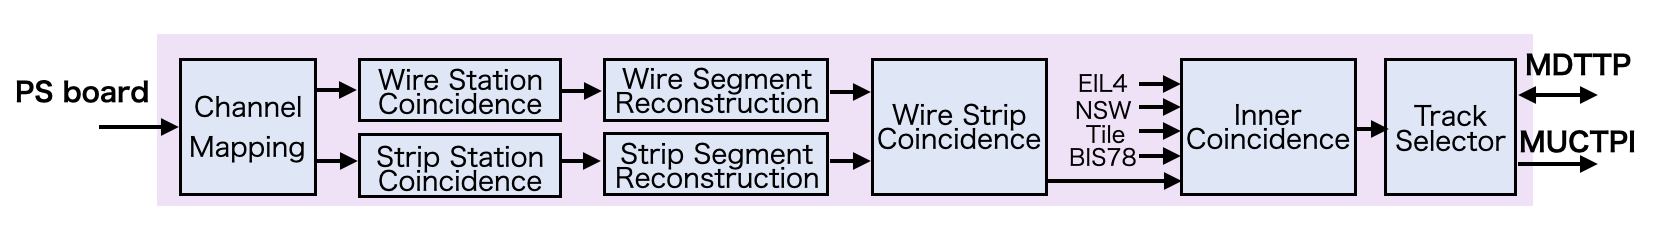
\includegraphics[width=16cm]{fig/SL/Trigger_over.png}
\caption[トリガー回路の全体像]{トリガー回路の全体像。高輝度LHC-ATLAS実験でのエンドキャップ部ミューオントリガー回路は、Channel Mapping、Station Coincidence、Segment Reconstruction、Wire Strip Coincidence、Inner Coincidence、Track Selectorという6段階のトリガー回路で構成される。}
\label{Trigger_over}
\end{figure}

Channel Mappingは、PS boardから受信したヒットデータをコインシデンスロジックの入力に適した形へと並び替える。Station Coincidenceはステーション内の2層または3層の間のコインシデンスをとり、そのステーションにおけるミューオンのヒット位置を表す"代表点"を出力する。Segment Reconstructionは各ステーションの代表点を組み合わせてミューオンの飛跡を再構成し、M3の代表点を基準点とした無限運動量飛跡とのなす角$\Delta\theta$、$\Delta\phi$を算出する。Wire Strip CoincidenceはWireで算出した$\Delta\theta$とStripで算出した$\Delta\phi$からミューオンの横方向運動量閾値\pt を概算する。TGC検出器に飛来するミューオンはエンドキャップトロイド磁場により、主に$\eta$方向に曲げられるため、$\Delta\theta$は\pt 再構成において有効な分別変数となる。一方、ミューオンは基本的には$\phi$方向に曲げられず、$\Delta\phi$はミューオンが衝突点から飛来したものであることを担保する目的で利用される。ここまでのトリガーロジックはTGC検出器からのヒットデータのみを利用するものであり、TGC BW Coincidenceと呼ぶ。Inner CoincidenceはTGC BW Coincidenceで再構成されたミューオン飛跡候補と、磁場内部の検出器(NSW、BIS78、RPC、EIL4 TGC、Tile カロリメーター)で得られたヒット情報の間でコインシデンスをとり、フェイクトリガーを削減するとともに\pt 精度の向上を図る。Inner Coincidenceまでのロジックは、1つの1/24セクターごとに最大112個のミューオン飛跡候補を出力する。Track Selectorは、112個のミューオン飛跡候補から\pt が大きい順に6つまで候補を絞り込む。そのうち3つはMDTTPに転送され、さらに高い精度で\pt が計算される。最終的に、MDTTPからSLに送り返された3つの飛跡候補と、MDTTPへ転送しなかった3つの飛跡候補を合わせてMUCTPIに送信する。

%ここまで

以下にそれぞれのロジックの概要と、論理回路への実装方法を説明する。

\subsection{Channel Mapping}
\subsubsection*{概要}
Channel MappingはPS board から受信するTGC BW 全チャンネルのヒット情報 (128 bit x 62 link) を、飛跡再構成に先んじてトリガー入力に適したフォーマットへとマッピングする。ここでは単にチャンネルを並び変えるだけでなく、TGC検出器のジオメトリーに合わせて設計されたフロントエンドのチャンネル構造を、トリガーロジックとして取り扱いやすいものへと変換する。TGC BW のエンドキャップ領域は$\eta$方向にM1は4つ、M2、M3は5つのチェンバーで構成されており、それぞれ不完領域がないようにオーバーラップを持って設置されている(図\ref{TGC_elec_mount}および図\ref{Channel_Mapping}参照)。オーバーラップするチャンネル同士はOR処理を施す。また、ストリップのコインシデンスではミューオンが$\eta$方向に曲げられ、複数のチェンバーに跨ってヒットを残した場合に対応するため、チェンバー間でコインシデンスをとる。例えば、図\ref{Channel_Mapping}に示す通り、M3の下から2つ目のチェンバーにヒットがある場合、M1、M2では下から1番目のチェンバーにヒットがある場合と、下から2番目にヒットがある場合が考えられる。どちらの場合でも、ステーション間でコインシデンスが取れるよう、M1及びM2では適切なチェンバー間でORをとる。

\begin{figure} 
\centering
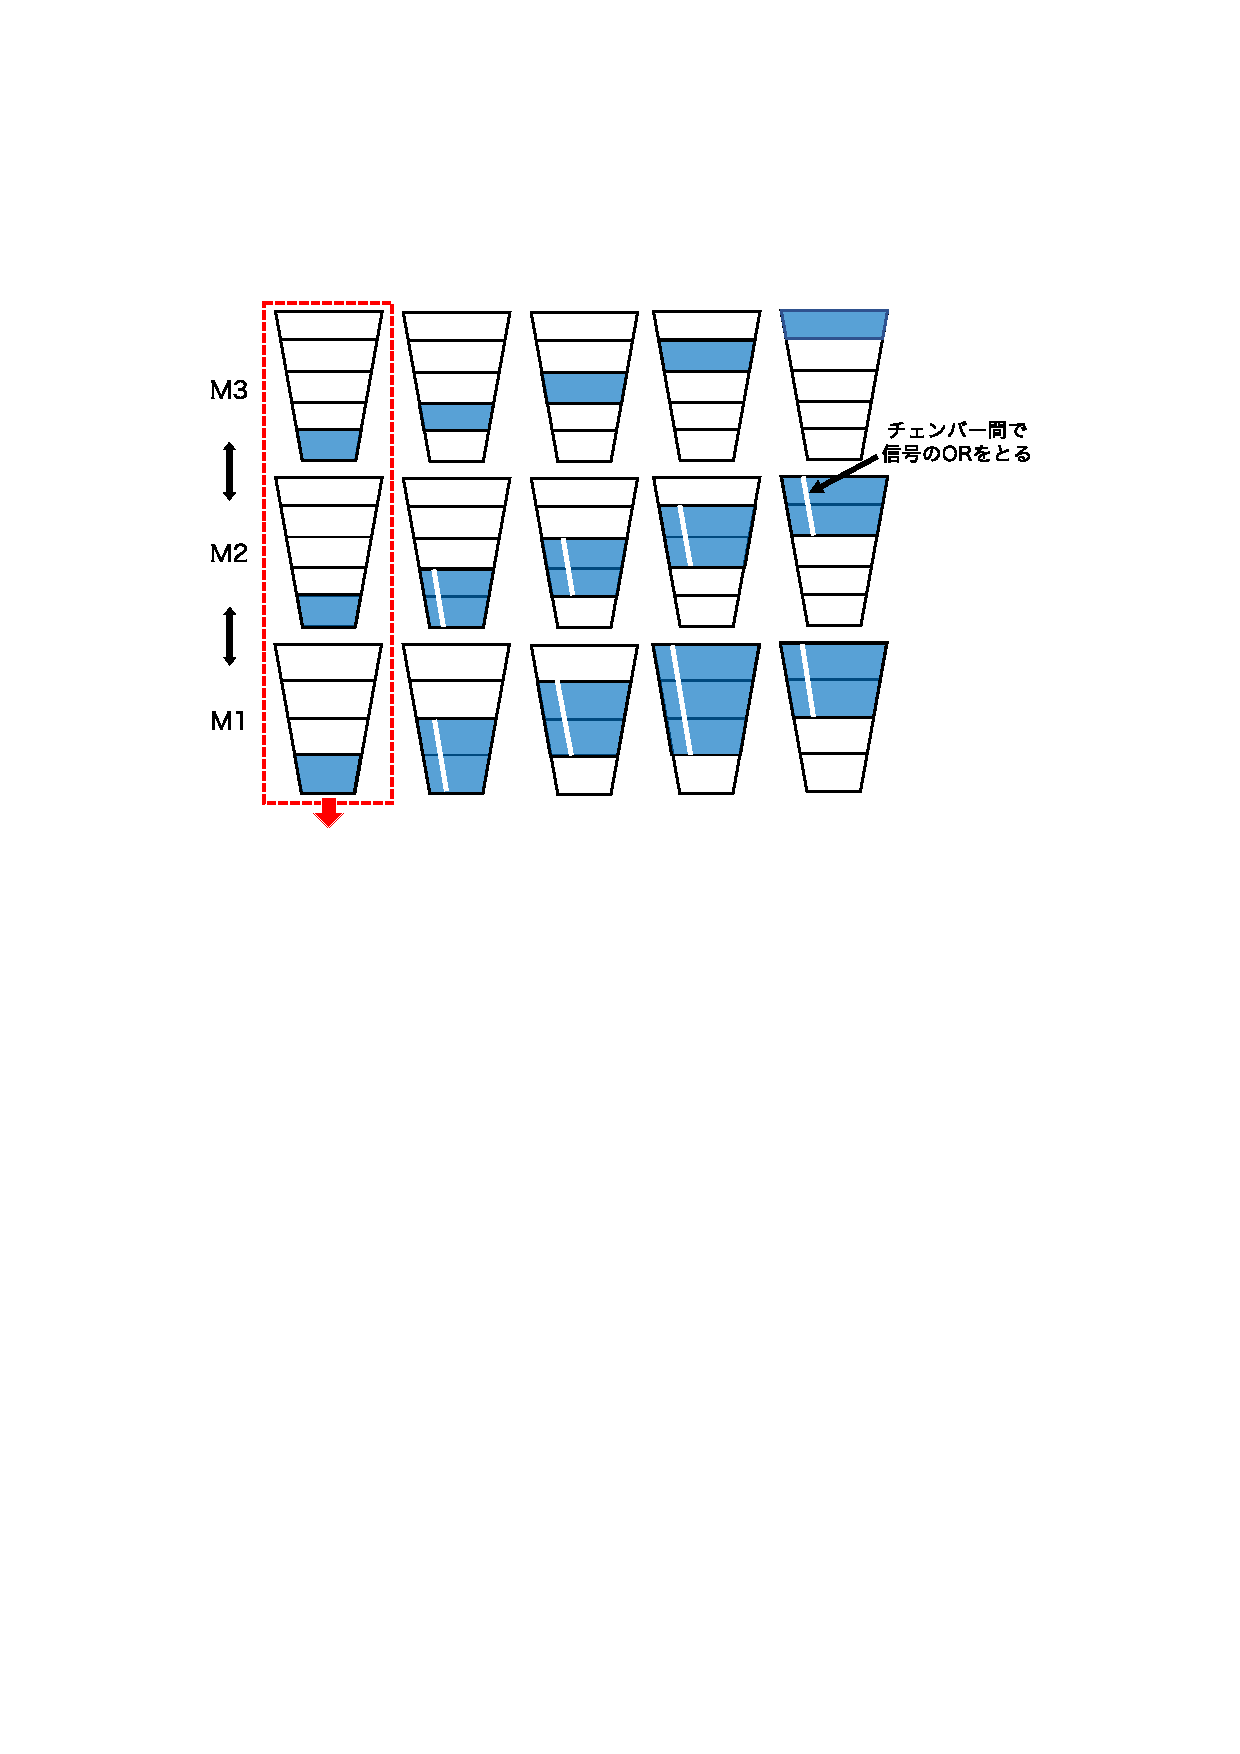
\includegraphics[width=16cm]{fig/SL/Channel_Mapping.pdf}
\caption[]{ストリップにおけるチェンバー間のORの取り方。M3チェンバーとのコインシデンスと担当するM1及びM2チェンバーでは、2つのチェンバー間でORをとった情報をStation Coincidenceの入力とする。\cite{mt_kawamoto}}
\label{Channel_Mapping}
\end{figure}

\subsubsection*{Channel Mapping の論理回路実装}
Channel Mappingモジュールは単純なワイヤーとOR回路で実装される。

\subsection{Station Coincidence}
\subsubsection*{概要}
図\ref{Concept_station}にStation Coincidenceの概要を示す\footnote{Station CoincidenceをIntra Station Coincidence、Segment Reconstruction を Inter Station Coincidenceと呼ぶ場合もある。}。TGC検出器はスタッガリング構造を取っており、ステーション内のワイヤーは互いに$\eta$方向にずらして、ストリップは互いに$\phi$方向にずらして設置されている。M1、M2、M3の各チャンネルが重複してカバーする$\eta$領域、$\phi$領域を代表点 ("Staggeredチャンネル") と呼ぶ。Station CoincidenceはM1の3層、M2の2層、M3の2層のヒットチャンネルを入力として、コインシデンスが取れた代表点を出力する。これによりデータ量を落としながら、より位置分解能を上げてミューオンのヒット位置を特定することができる。

\begin{figure} 
\centering
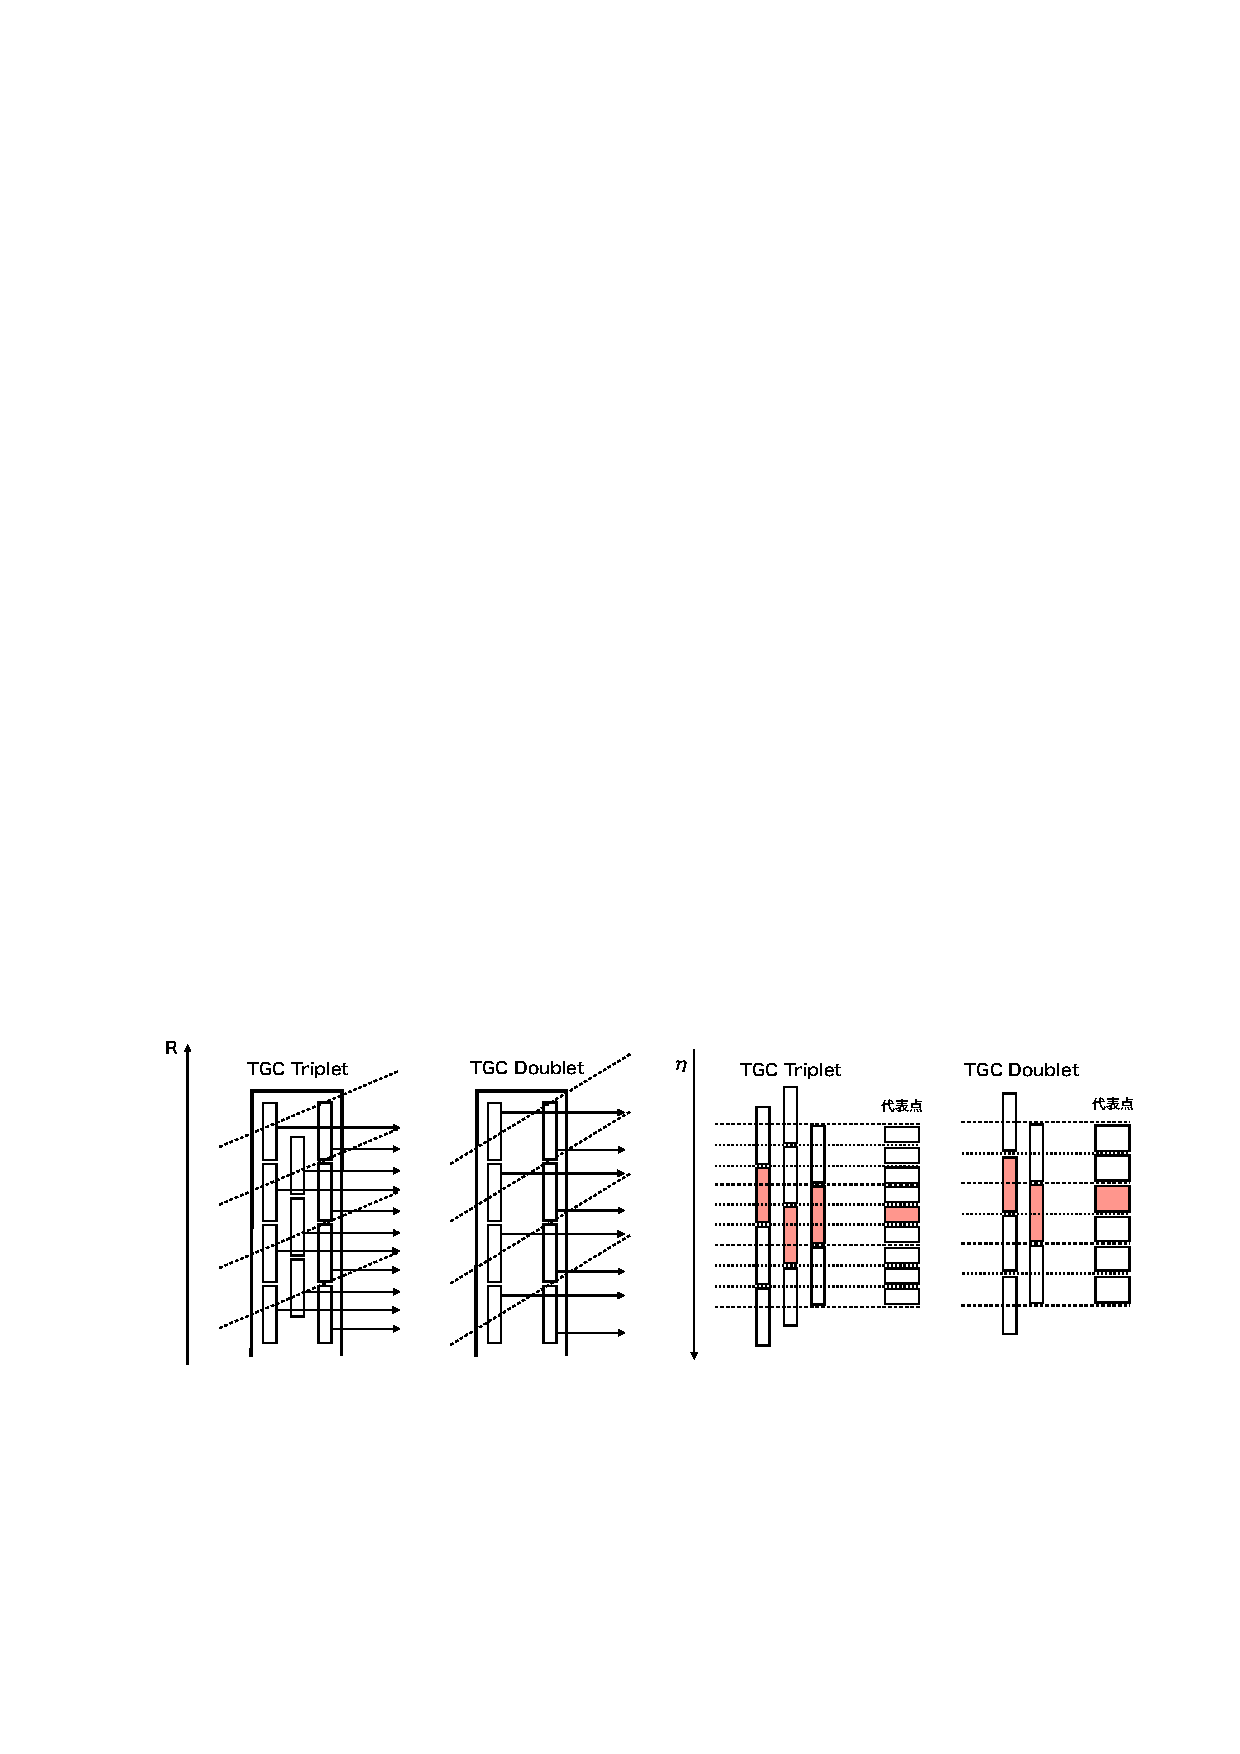
\includegraphics[width=16cm]{fig/SL/Concept_station.pdf}
\caption[Station コインシデンスの概要]{Station Coincidence の概要\cite{mt_mino}。TGC検出器ではステーション内のワイヤーは$\eta$方向に、ストリップは$\phi$方向にずらして設置されており、各層のチャンネルが重複してカバーsる$\eta$領域を代表点として定義する。Station Coincidenceでは2層または3層でコインシデンスのとれた代表点を出力する。}
\label{Concept_station}
\end{figure}

\subsubsection*{Wire Station Coincidenceの論理回路実装}
このモジュールの駆動クロックは、LHCバンチ交差クロックに同期した40 MHzクロックで、レイテンシーは1クロックチック ( 25 ns )である。M1ステーションにおけるコインシデンスロジックの概要を図\ref{StationCoin_wire}に示す。ステーションコインシデンスはAND回路とOR回路の組み合わせ回路として実装される。3層中3層にヒットがあった場合に代表点を出力する3/3コインシデンス、2層にヒットがあった場合の2/3コインシデンス、1層にヒットがある場合の1/3コインシデンスが独立に用意されており、それぞれが並列に動作する。

\begin{figure} 
    \centering
    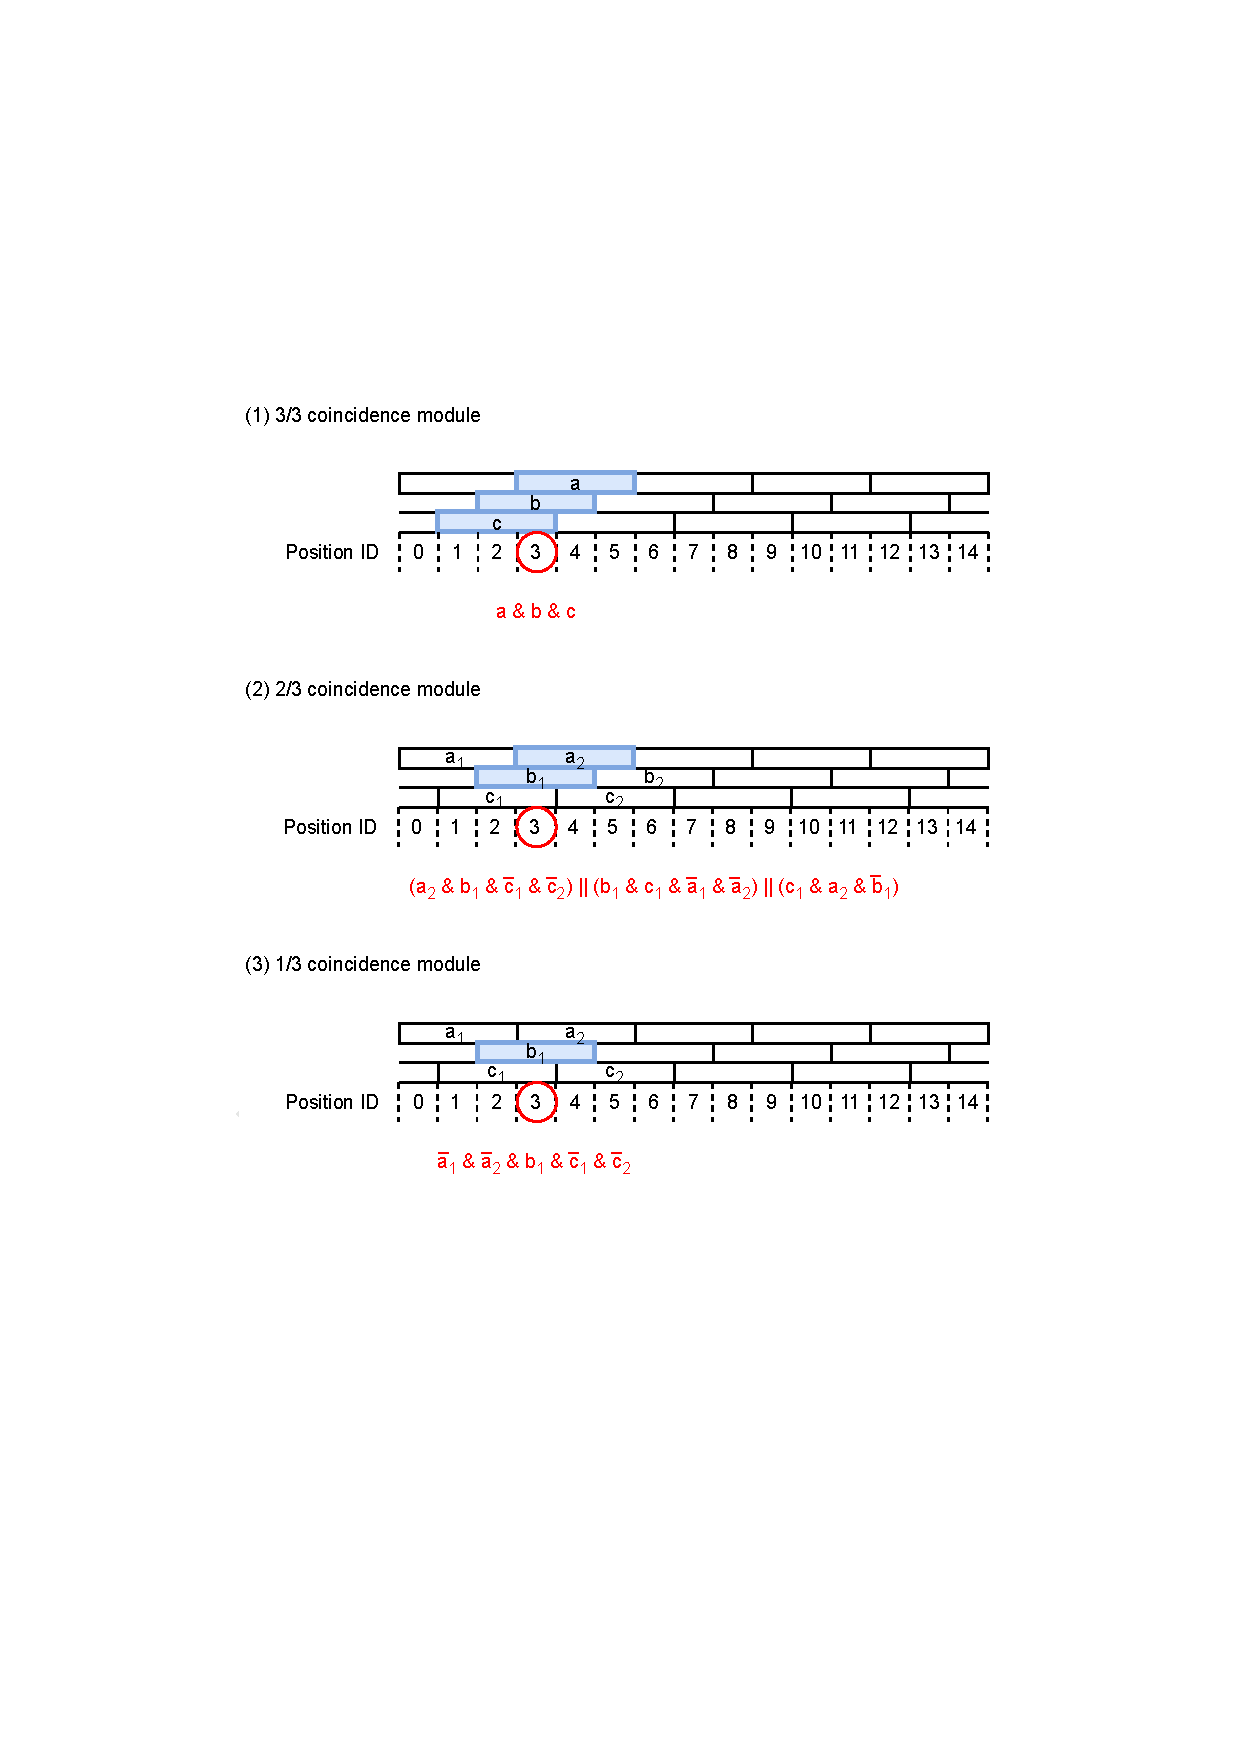
\includegraphics[width=16cm]{fig/SL/StationCoin_wire.pdf}
    \caption[M1 tripletにおけるコインシデンスロジック]{M1 tripletにおけるコインシデンスロジック\cite{SLPDR}。3層中3層にヒットがあった場合に代表点を出力する3/3コインシデンス、3層中2層の場合に代表点を出力する2/3コインシデンス、3層中1層の場合に代表点を出力する1/3コインシデンスが用意されている。}
    \label{StationCoin_wire}
\end{figure}

M2、M3ステーションは2層で構成されているため、2/2コインシデンスと1/2コインシデンスが用意されており、それぞれのロジックは図\ref{StationCoin_doublet}のように実装される。
    
\begin{figure} 
\centering
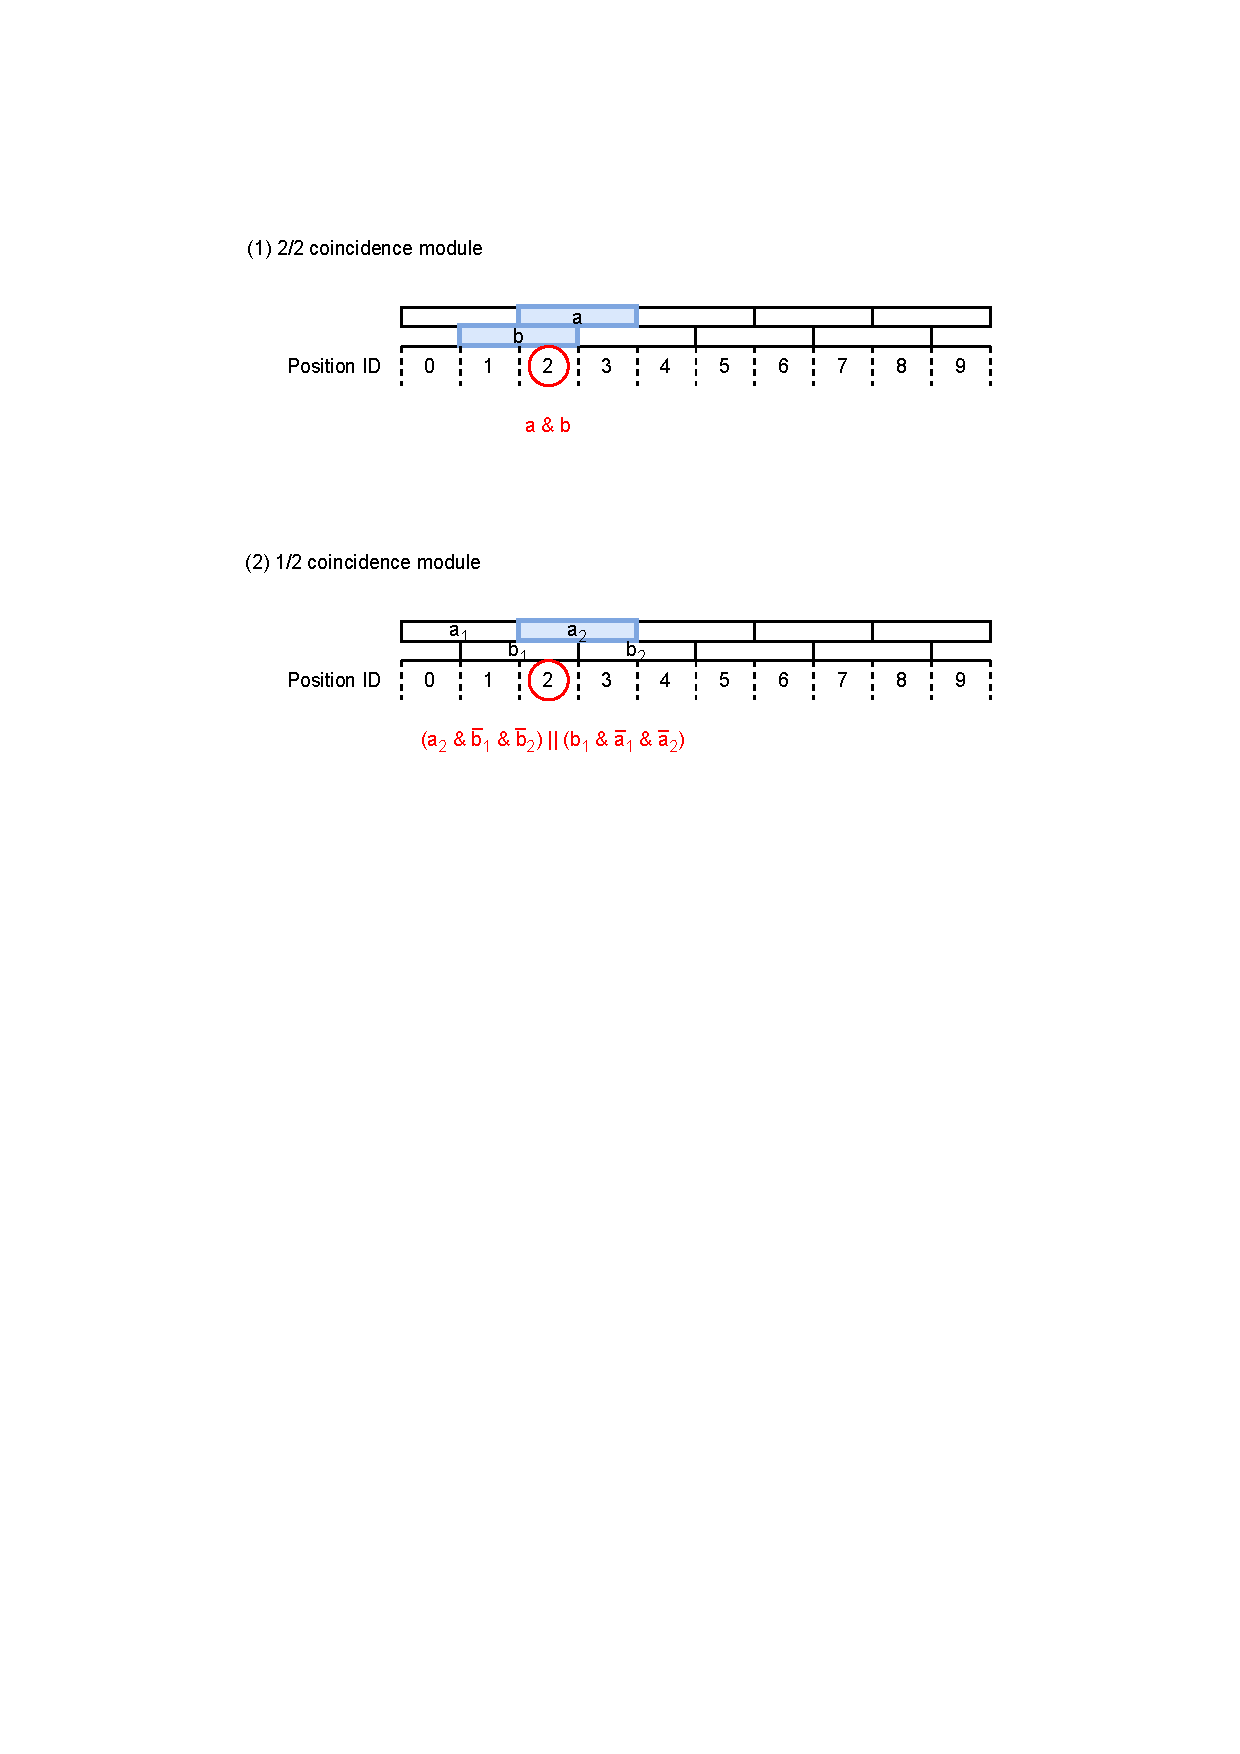
\includegraphics[width=16cm]{fig/SL/StationCoin_doublet.pdf}
\caption[M2・M3 ステーションにおけるコインシデンスロジック]{M2、M3 ステーションにおけるコインシデンスロジック\cite{SLPDR}。2層中2層にヒットがあった場合に代表点を出力する2/2コインシデンス、2層中1層の場合に代表点
を出力する1/2コインシデンスが用意されている。}
\label{StationCoin_doublet}
\end{figure}

各コインシデンスロジックで、複数の代表点が出力された場合には各サブユニットごとに後段に送る代表点を選別する。M1、M2ステーションでは検出器がユニットの中心により近いものが2つ、M3ステーションでは$\eta$がより小さいものが1つ選ばれる。
% ステーションコインシデンスの最終的な出力は図\ref{}のテーブルのようにまとめらる。

\subsubsection*{Strip Station Coincidenceの論理回路実装}
このモジュールの駆動クロックは、LHCバンチ交差クロックに同期した40 MHzクロックで、レイテンシーは1クロックチック ( 25 ns )である。コインシデンスのロジックは基本的にワイヤーと同じで、M1、M2、M3ともに2層構造になっているためそれぞれ2/2、1/2ロジックが並列に走っている。
% 最終的な出力は図\ref{}のようにまとめられ、後段に送られる。


\subsection{Segment Reconstruction}
\label{subsec:segment_reco}
\subsubsection*{概要}
Segment ReconstructionではStation Coincidenceで得られた、各ステーションの代表点の組み合わせから、無限運動量飛跡と実際の飛跡のなす角度 ($\Delta\theta$、$\Delta\phi$)を算出する。ミューオンはエンドキャップトロイド磁場により主に$\eta$方向に曲げられるため、$\Delta\theta$は\pt を再構成する上で有効な分別変数となる。一方、$\phi$方向にはほとんど曲げられず、有効な分別変数とはなり得ない。ミューオンが衝突点から飛来したものであることを担保するための、追加的な条件として利用される。Segment Reconstructionの概念図を図\ref{Concept_segment}に示す。角度情報の概算には、パターンマッチングと呼ばれる手法を用いる。この手法ではあらかじめ、代表点の組み合わせとそこから計算される角度情報の対応関係をまとめたテーブル (パターンリスト、LUTともよぶ) を用意することで、複雑な計算をせずに高速で角度情報を再構成する。

\begin{figure} 
\centering
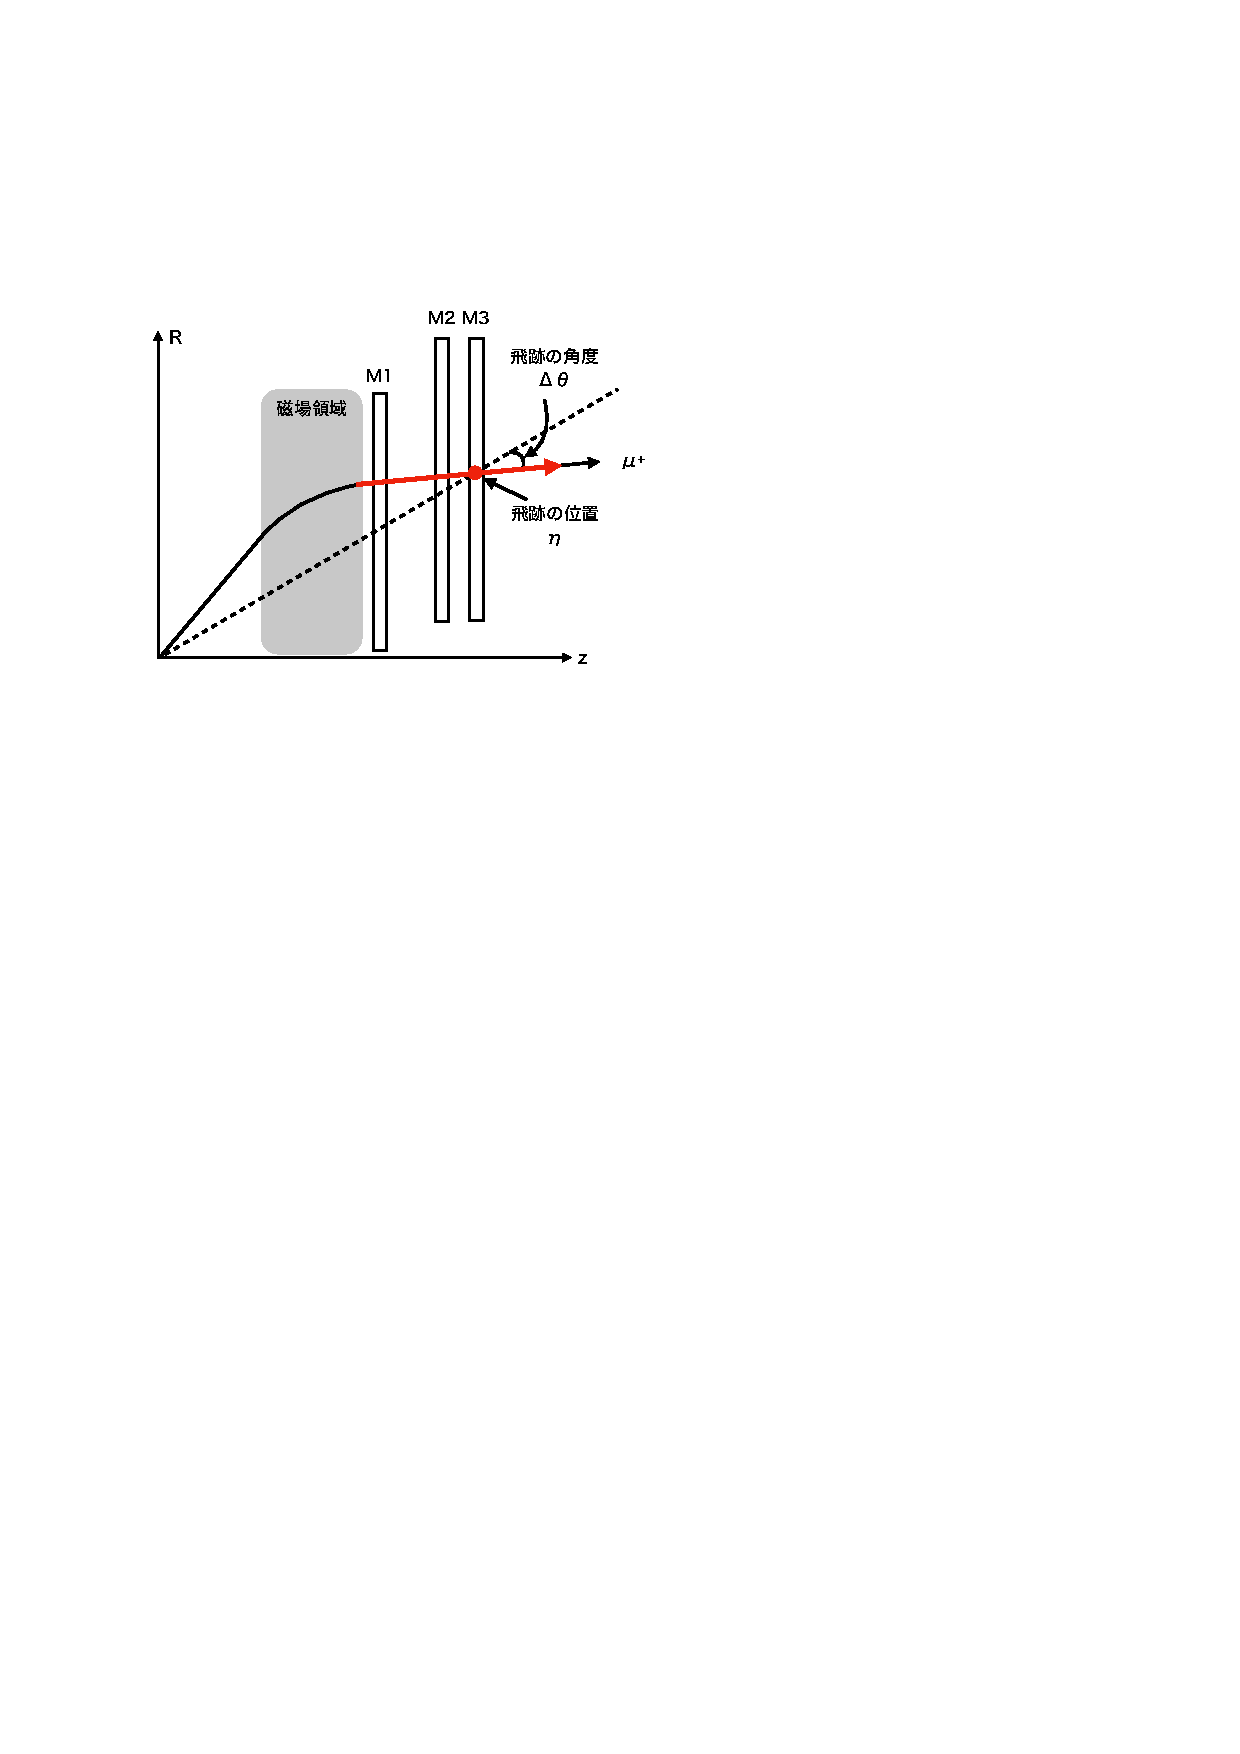
\includegraphics[width=12cm]{fig/SL/Concept_segment.pdf}
\caption[Segment Reconstructionのコンセプト]{$\eta$方向のパターンマッチングの概念図\cite{mt_mino}。黒い線が実際のミューオンの飛跡を表し、赤い線がTGCのヒットから再構成される飛跡を表す。黒い点線はM3ステーションの代表点と衝突点を結んだ、無限運動量飛跡を表す。M1、M2、M3の代表点の組み合わせから、実際の飛跡と無限運動量飛跡とがなす角度$\Delta\theta$を再構成する。}
\label{Concept_segment}
\end{figure}

\subsubsection*{Wire Segment Reconstructionの論理回路実装}
このモジュールの駆動クロックは、LHC クロックに同期した周波数 160 MHz のクロックで、レイテンシーは 12 クロックチック分 (75 ns) である。

Wire Segment ReconstructionはUnit、Subunitと呼ばれる単位領域でトリガーセクターを分割して、Subunitごとに並列にコインシデンスロジックを用意する。ワイヤーロジックではエンドキャップ領域を37分割、フォワード領域を16分割したものをUnitと定義する。図\ref{StationCoin_unit}にユニットの構造を示す。1つのユニットはM1ステーションの96 代表点、M2ステーションの32 代表点、M3ステーションの16 代表点をカバーする。また、1つのユニットを4等分するようにSubunitが定義されており、Subunitに1つパターンマッチング用のLUTが用意される。UnitやSubunitの大きさは必要なLUTのサイズによる制約で決められており、FPGAのRAMリソースに合わせて最適化されている。Unitの範囲は、とあるM3チャンネルにヒットを残した \pt$\,$5 GeVのミューオンを再構成するのに必要な、M1、M2チャンネルを網羅するよう定義された。

\begin{figure} 
    \centering
    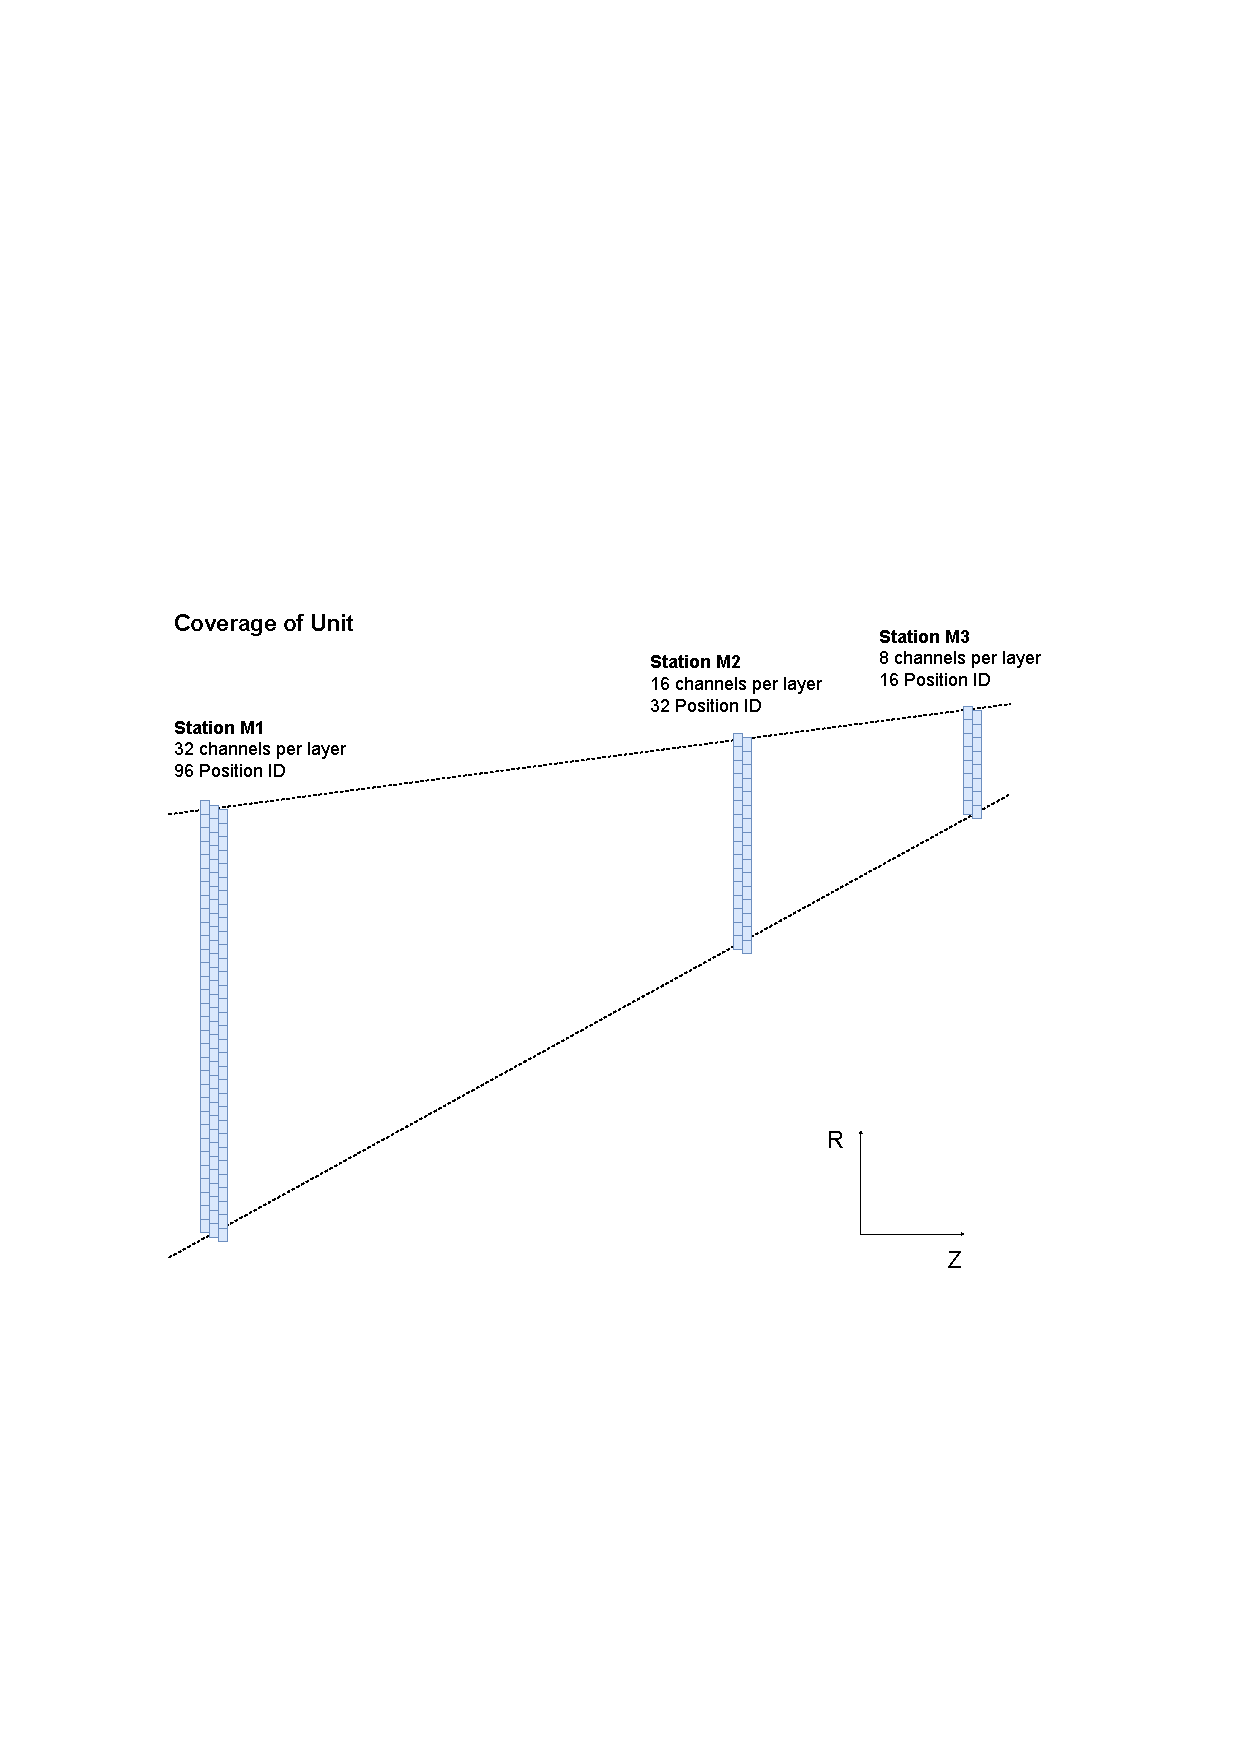
\includegraphics[width=12cm]{fig/SL/StationCoin_unit.pdf}
    \caption[Wire Segment Reconstruction におけるユニット]{Wire Segment Reconstruction におけるユニット。1つのユニットはM1の96代表点、M2の32代表点、M3の16代表点をカバーする。\cite{SLPDR}}
    \label{StationCoin_unit}
\end{figure}

最終的にはそれぞれのサブユニットから最大1つの飛跡情報を出力するため、SL全体では最大360の飛跡候補が出力される。Wire Segment Reconstructionの各サブユニット内でのロジックの概要を図\ref{SegReco_wire}に示す。各サブユニットはAddress Specifier・Segment Extractor・Segment Selector で構成される。以下でそれぞれのモジュールについて述べる。

\begin{figure} 
\centering
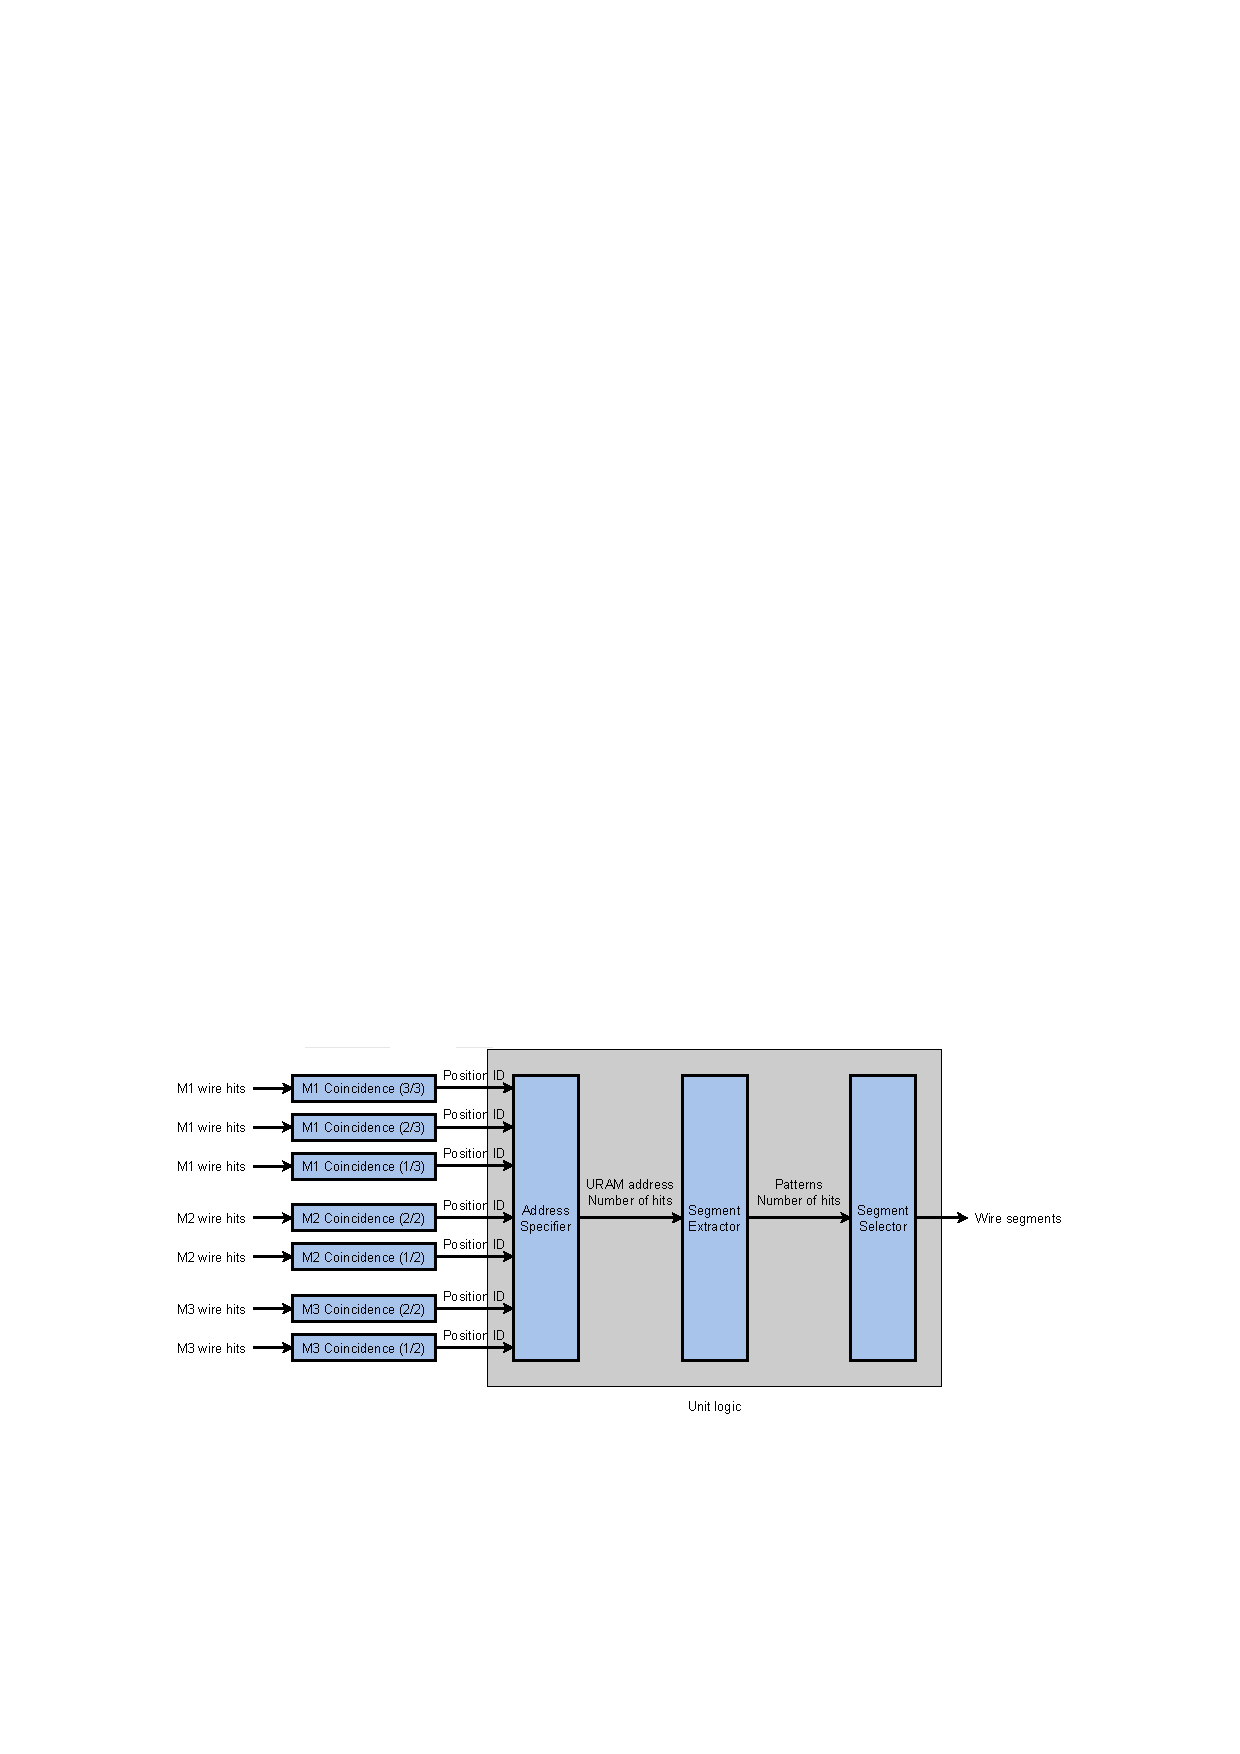
\includegraphics[width=16cm]{fig/SL/SegReco_wire.pdf}
\caption[Wire Segment Reconstructionのブロックダイアグラム]{Wire Segment Reconstructionのブロックダイアグラム\cite{SLPDR}。Wire Segment Reconstructionは、Station Coincidenceで得られた代表点の組み合わせから、LUTのアドレスを作成するAddress Specifier、LUTから対応するデータを取り出すSegment Extractor、Segment Extractorから得られる最大8つの飛跡候補から後段に送る1つを選別するSegment Selectorで構成される。}
\label{SegReco_wire}
\end{figure}

\subsubsection*{Address Specifier}
Wire Station Coincidenceで得られた各ステーションの代表点を組み合わせて、LUT にアクセスするためのアドレスを作成する。1つのSubunitはStation Coincidence から M1の代表点を最大6つ、M2のものを最大4つ、M3のものを最大2つ、それぞれ受け取るため、M1、M2、M3の代表点の組み合わせは最大$6 \times 4 \times 2 = 48$ パターン存在する。Address Specifierはこの中から8パターンを選抜してSegment Extractorへ送る。パターンを選択する際にはマッチレイヤーが多いもの優先する。具体的に優先順位を定めたテーブルを表\ref{tab:StationCoin_wire}に示す。より上位にリストされているコインシデンスパターンが優先して送られる。また同率の組み合わせが複数存在する場合には、$\eta$がより小さいものが選ばれる。なお、同表中のFractionの値はレイヤーあたりの検出効率を94 \%と仮定して算出したものである。

\begin{table}[h]
    \centering
    \caption{Wire Station Coincidenceにおけるコインシデンスパターン}
    \label{tab:StationCoin_wire}
    \begin{tabular}{|cc|c|}
    \hline
    \multicolumn{1}{|c|}{\multirow{2}{*}{Coincidence Pattern}} & Hit Pattern & \multirow{2}{*}{Faraction} \\ \cline{2-2}
    \multicolumn{1}{|c|}{}                                     & M1 M2 M3    &                            \\ \hline\hline
    \multicolumn{1}{|c|}{7/7}                                  & 3/3 2/2 2/2 & 0.649                      \\ \hline
    \multicolumn{1}{|c|}{6/7A}                                 & 2/3 2/2 2/2 & 0.124                      \\ \hline
    \multicolumn{1}{|c|}{6/7B}                                 & 3/3 1/2 2/2 & 0.083                      \\ \hline
    \multicolumn{1}{|c|}{6/7C}                        & 3/3 2/2 1/2 & 0.083                      \\ \hline
    \multicolumn{1}{|c|}{5/7A}                                 & 2/3 1/2 2/2 & 0.016                      \\ \hline
    \multicolumn{1}{|c|}{5/7B}                                 & 1/3 2/2 1/2 & 0.016                      \\ \hline
    \multicolumn{1}{|c|}{5/7C}                                 & 3/3 1/2 1/2 & 0.011                      \\ \hline
    \multicolumn{1}{|c|}{5/7D}                                 & 1/3 2/2 2/2 & 0.008                      \\ \hline\hline
    \multicolumn{2}{|c|}{Total}                                              & 0.988                      \\ \hline
    \end{tabular}
\end{table}

\subsubsection*{Segment Extractor}
Wire Segment Reconstructionで利用されるLUTはFPGAのURAM上に格納される。Segment ExtractorではAddress Specifierで作られたアドレスをもとに、URAMにアクセスし、対応するデータ (Wire Segment ) を出力する。Wire Segmentのデータフォーマットを表\ref{tab:WireSegment}に示す。URAMはdual portで設計されており、1つのサブユニットが2ポート利用する。そのため1つのサブユニットは40 MHz クロック 1チックの間で 8つのデータを処理する。

\begin{table}[h]
    \centering
    \caption{Wire Segmentのフォーマット}
    \label{tab:WireSegment}
    \begin{tabular}{|c|c|}
    \hline
    \# of bits & Name                                                                       \\ \hline\hline
    1          & Flag of successful reconstruction                                          \\ \hline
    2          & Number of the stations with hits used for coincidence                      \\ \hline
    8          & Angle difference $\Delta\theta$ between the segment and the vector from IP \\ \hline
    12         & Global $\eta$ position of the segment                                      \\ \hline
    \end{tabular}
\end{table}

\subsubsection*{Segment Selector}
Segment Extractorから送られる最大8つのWire Segment から マッチレイヤーの多さを基準に最大1つ選択して、Wire Strip Coincidence へと送信する。マッチレイヤーも同じものが複数ある場合には$\Delta\theta$がより小さいものを選ぶ。

\subsection*{Strip Segment Reconstruction}
このモジュールの駆動クロックは、LHC クロックに同期した周波数 240 MHz のクロックで、レイテンシーは 21 クロックチック分 (87.5 ns) である。
Strip Segment ReconstructionもUnit、Subunit呼ばれる単位領域でトリガーセクターを分割して、Subunitごとに並列にコインシデンスロジックを用意する。Strip では 1つのチェンバーを4分割するようユニットが定義される。エンドキャップ領域は5枚のチェンバーで構成されるため20 Unit、フォワード領域は1枚のチェンバーで構成されるため5 unit 存在する。図\ref{StationCoin_unit_strip}にユニットの構造を示す。1つのユニットはM1ステーションの40 代表点、M2ステーションの 24代表点、M3ステーションの 16代表点をカバーする。また、1つのユニットを2等分するようにSubunitが定義されており、Subunitに1つパターンマッチング用のLUTが用意される。

\begin{figure} 
    \centering
    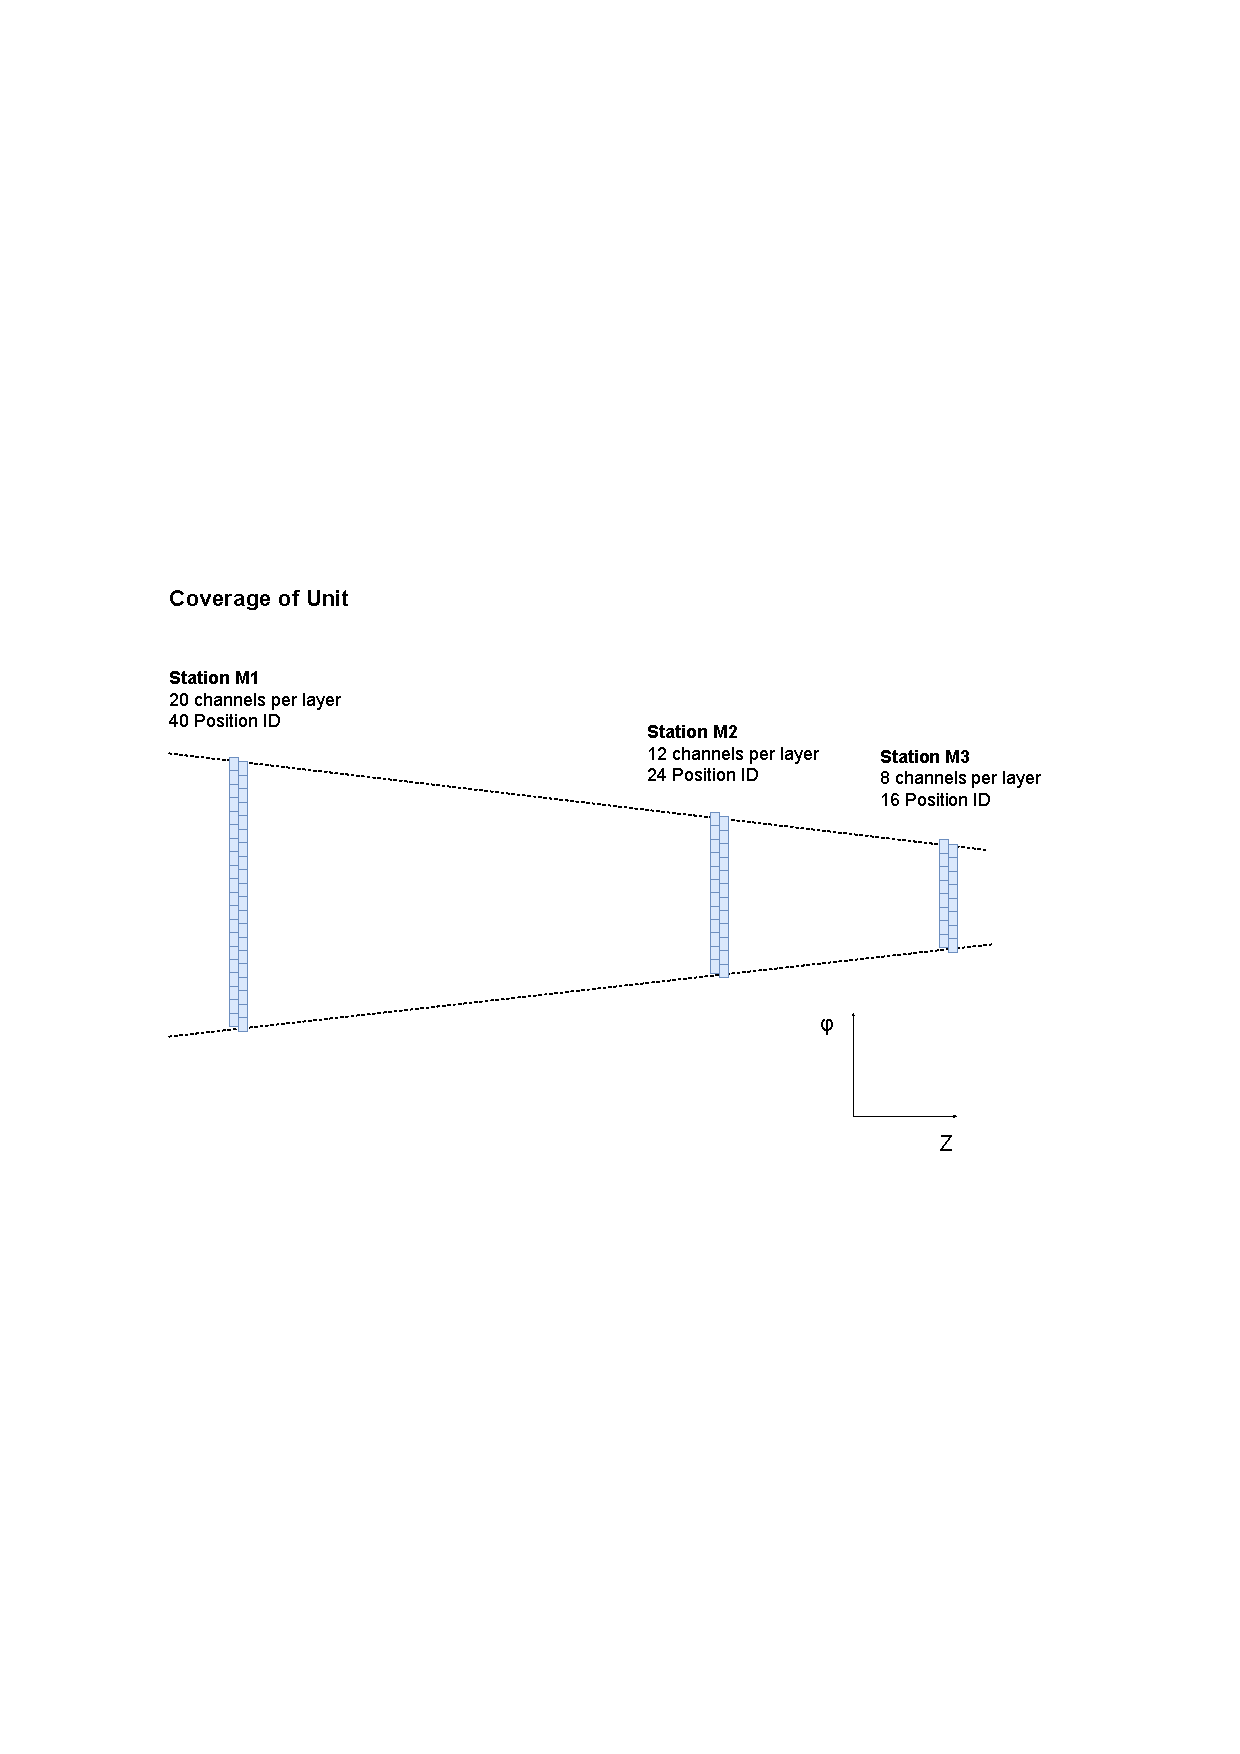
\includegraphics[width=12cm]{fig/SL/StationCoin_unit_strip.pdf}
    \caption[Strip Segment Reconstruction におけるユニット]{Strip Segment Reconstruction におけるユニット\cite{SLPDR}。1つのユニットはM1の40代表点、M2の24代表点、M3の16代表点をカバーする。}
    \label{StationCoin_unit_strip}
\end{figure}

Strip Segment Reconstructionではサブユニットごとに1つLUTが用意され、サブユニット内の代表点を組み合わせることでパターンマッチングを行う。最終的にはユニット内の2つのサブユニット合わせて、1つの角度情報が出力される。SL全体では最大45の飛跡情報が出力される。Strip Segment Reconstructionの各サブユニット内でのロジックの概要を図\ref{SegReco_strip}に示す。各サブユニットはAddress Specifier・Segment Extractor・Segment Selector で構成される。以下でそれぞれのモジュールについて述べる。

\begin{figure} 
\centering
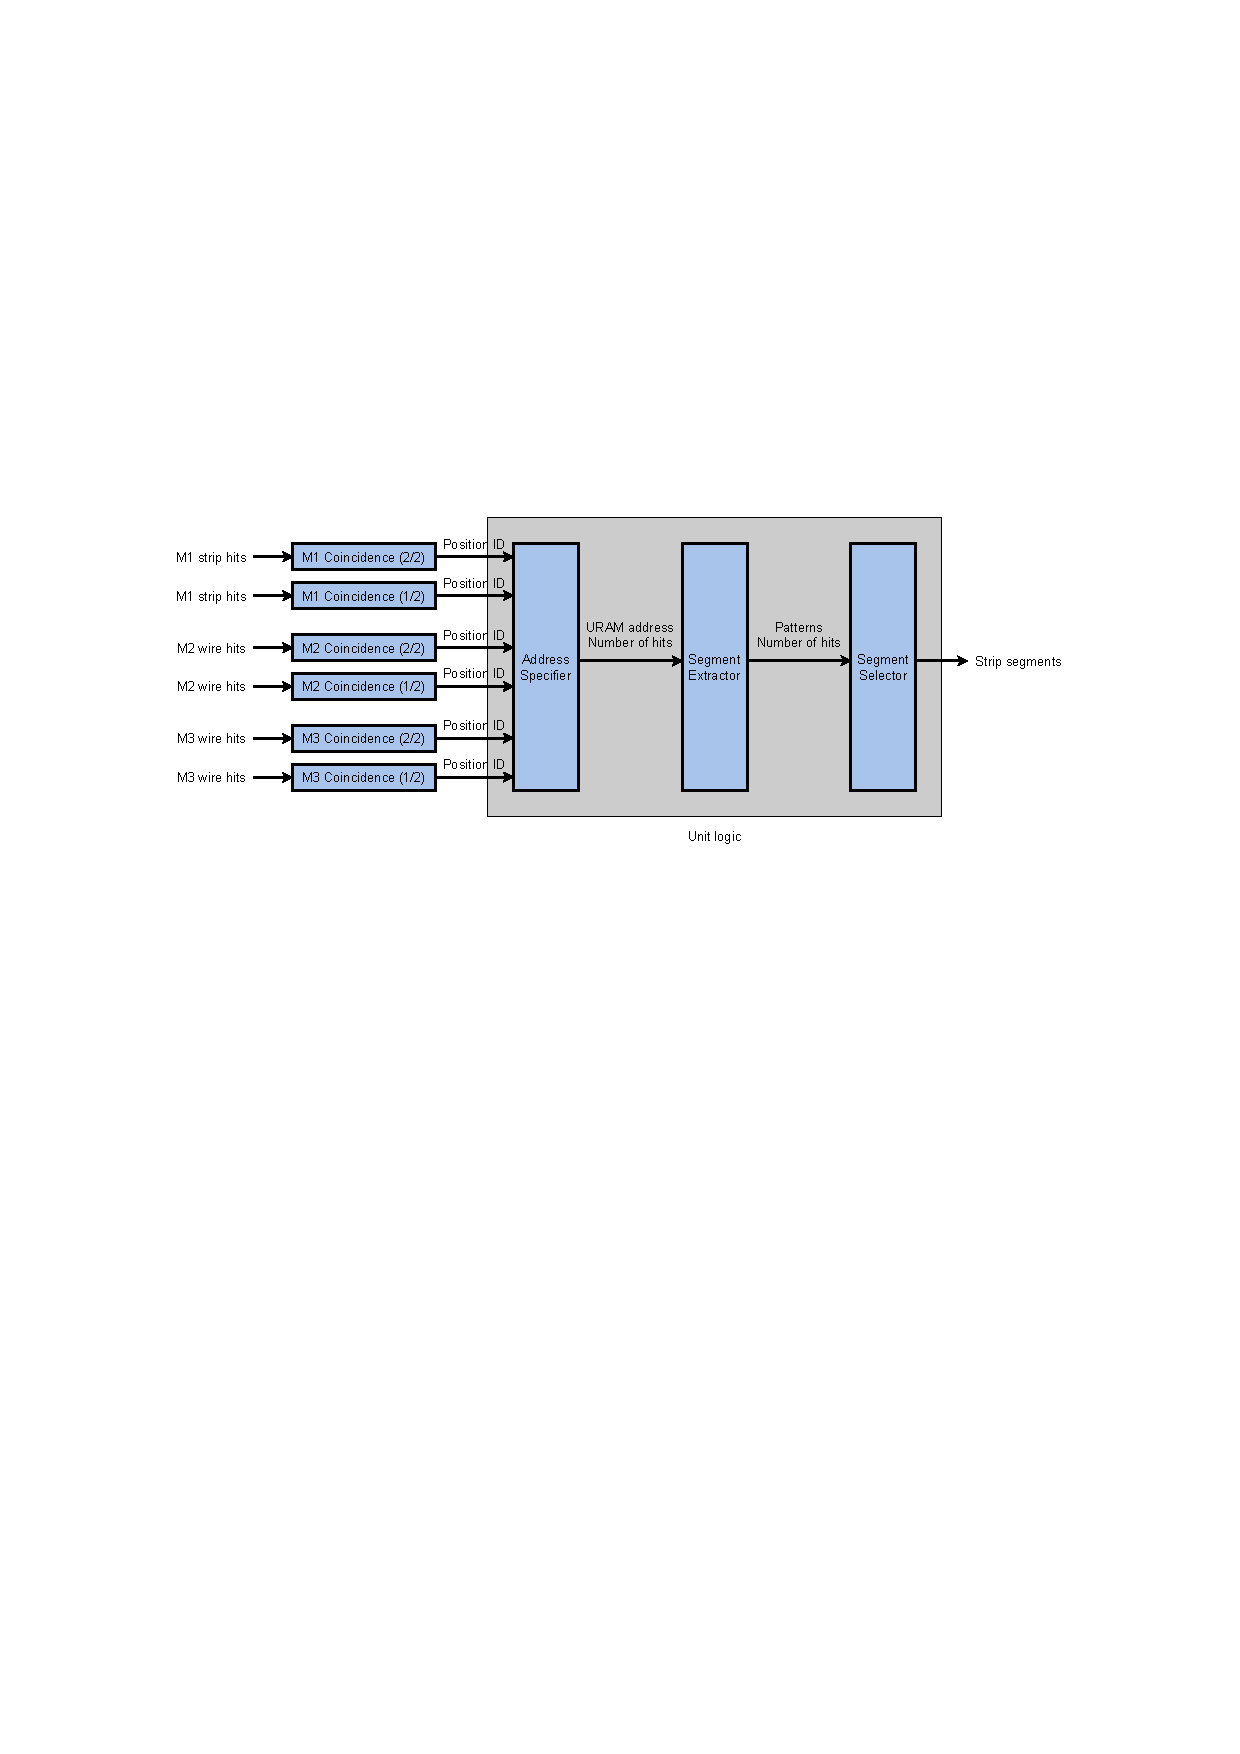
\includegraphics[width=16cm]{fig/SL/SegReco_strip.pdf}
\caption[Strip Segment Reconstruction のブロックダイアグラム]{Strip Segment Reconstruction のブロックダイアグラム\cite{SLPDR}。Strip Segment Reconstructionは、Station Coincidenceで得られた代表点の組み合わせから、LUTのアドレスを作成するAddress Specifier、LUTから対応するデータを取り出すSegment Extractor、Segment Extractorから得られる最大6つの飛跡候補から後段に送る1つを選別するSegment Selectorで構成される。}
\label{SegReco_strip}
\end{figure}

\subsubsection*{Address Specifier}
Strip Station Coincidenceで得られた各ステーションの代表点を組み合わせて、LUT にアクセスするためのアドレスを作成する。
1つのSubunitはStation Coincidence から M1の代表点を最大4つ、M2のものを最大4つ、M3のものを最大2つ、それぞれ受け取るため、M1、M2、M3の代表点の組み合わせは最大$4 \times 4 \times 2 = 32$ パターン存在する。Address Specifierはこの中から6つのパターンを選抜してSegment Extractorへ送る。パターンを選択する際にはワイヤーのロジックと同様にマッチレイヤーが多いもの優先する。具体的に優先順位を定めたテーブルを表\ref{tab:SegmentReco_strip}に示す。

\begin{table}[]
    \centering
    \caption{Strip Segment Reconstructionにおけるwire segmentのデータフォーマット}
    \label{tab:SegmentReco_strip}
    \begin{tabular}{|cc|}
    \hline
    \multicolumn{1}{|c|}{\multirow{2}{*}{Coincidence Pattern}} & Hit Pattern \\ \cline{2-2} 
    \multicolumn{1}{|c|}{}                                     & M1 M2 M3    \\ \hline\hline
    \multicolumn{1}{|c|}{6/6}                                  & 2/2 2/2 2/2 \\ \hline
    \multicolumn{1}{|c|}{5/6A}                                 & 2/2 1/2 2/2 \\ \hline
    \multicolumn{1}{|c|}{5/6B}                                 & 1/2 2/2 2/2 \\ \hline
    \multicolumn{1}{|c|}{5/6C}                                 & 2/2 2/2 1/2 \\ \hline
    \multicolumn{1}{|c|}{4/6A}                                 & 1/2 1/2 2/2 \\ \hline
    \multicolumn{1}{|c|}{4/6B}                                 & 2/2 1/2 1/2 \\ \hline
    \multicolumn{1}{|c|}{4/6C}                                 & 1/2 2/2 1/2 \\ \hline\hline
    \multicolumn{2}{|c|}{Total}                                              \\ \hline
    \end{tabular}
\end{table}

\subsubsection*{Segment Extractor}
Strip Segment Reconstructionで利用されるLUTはFPGAのURAM上に格納される。Segment ExtractorではAddress Specifierで作られたアドレスをもとに、URAMにアクセスし、対応するデータ ( Strip Segment ) を出力する。Strip Segmentのデータフォーマットを表\ref{tab:StripSegment}に示す。URAMはdual portで設計されており、2つのサブユニットが1ポートずつ利用する。そのため1つのサブユニットは、40 MHzクロック 1チックの間に6つのデータを処理する。

\begin{table}[]
    \centering
    \caption{Strip Segmentのフォーマット}
    \label{tab:StripSegment}
    \begin{tabular}{|c|c|}
    \hline
    \# of bits & Name                                                                     \\ \hline\hline
    2          & Number of the stations with hits used for coincidence                    \\ \hline
    6          & Local $\phi$ position in the chamber                                     \\ \hline
    9          & Angle difference $\Delta\phi$ between the segment and the vector from IP \\ \hline
    \end{tabular}
\end{table}

\subsubsection*{Segment Selector}
Segment Extractorから送られる最大6つのStrip Segment から マッチレイヤーの多さを基準にユニットごとに最大1 Segment 選択して、Wire Strip Coincidence へと送信する。マッチレイヤーも同じものが複数ある場合には$\Delta\phi$がより小さいものを選ぶ。

\subsection{Wire-Strip Coincidence}
\subsubsection*{概要}
Wire Strip CoincidenceではWire Segment Reconstructionで算出した$\Delta\theta$とStrip Segment Reconstructionで算出した$\Delta\phi$を組み合わせることで、横方向運動量 \pt を概算する。\pt の計算もCoincidence Windowと呼ばれるLUTを用いて行う。Coincidence Windowの例を図\ref{Concept_WS}に示す。

\begin{figure} 
\centering
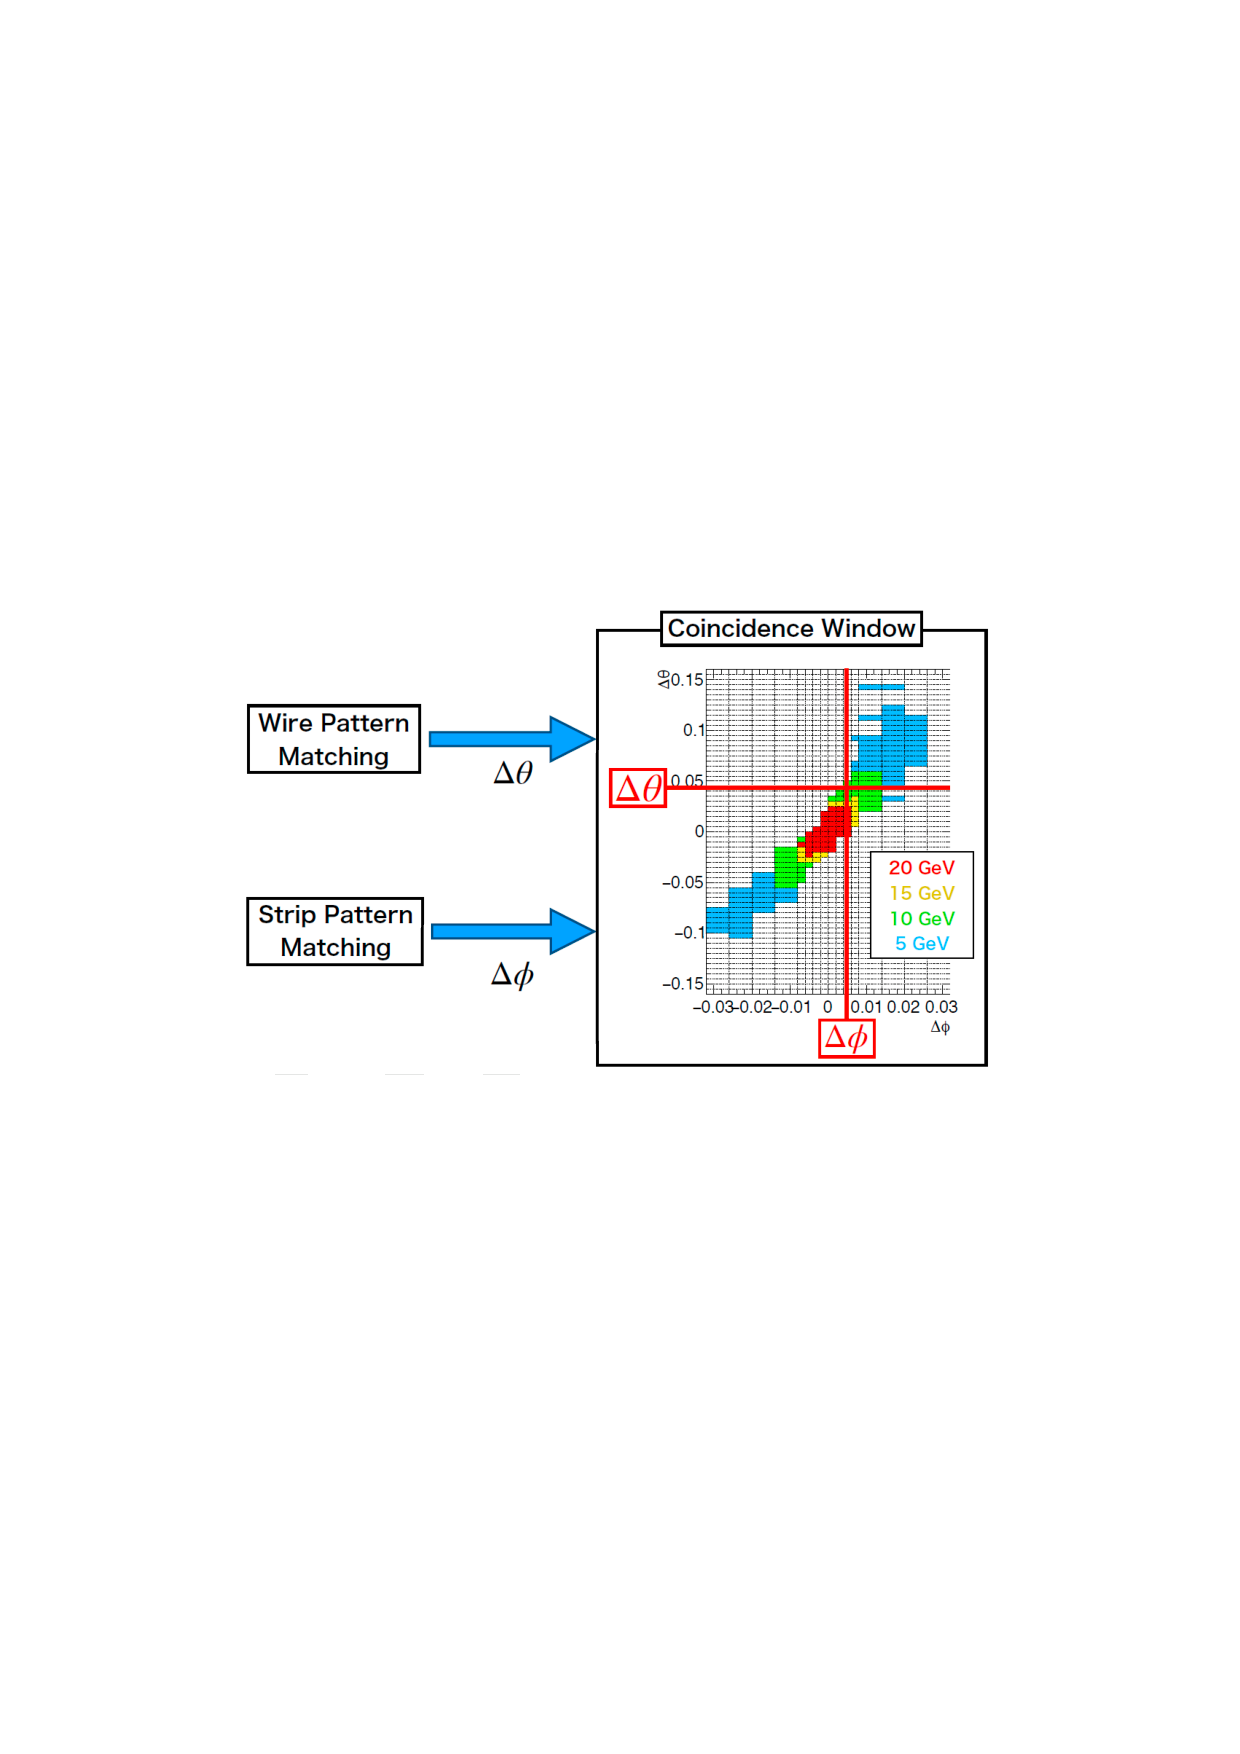
\includegraphics[width=16cm]{fig/SL/Concept_WS.pdf}
\caption[Wire Strip CoincidenceにおけるCoincidence Windowの例]{Wire Strip CoincidenceにおけるCoincidence Windowの例\cite{SLPDR}。WireおよびStrip Segment Reconstructionで再構成された$\Delta\theta$、$\Delta\phi$から$p_\mathrm{T}$閾値を概算する。$\Delta\phi$で再構成したミューオンが衝突点に由来するものであることを担保し、$\Delta\theta$で\pt を決めている。$\Delta\phi$の値域が$\Delta\theta$の関数になっているのは、この例で示した領域が荷電粒子を$\phi$方向にも曲げる磁場を持つ例外的な点であるためである。現状\pt は5 GeV、10 GeV、15 GeV、20 GeVの4段階で出力している。本番運用時には4 bit、16段階で出力する予定である。}
\label{Concept_WS}
\end{figure}

\subsubsection*{Wire Strip Coincidenceの論理回路実装}
駆動クロックはLHCバンチ交差クロックに同期した160 MHzクロックで、レイテンシーは6クロックチック分 (37.5 ns)である。
Wire Strip Coincidenceでは Region と呼ばれる単位領域を新たに設定し、Regionごとに並列にコインシデンスロジックを走らせる。Regionは後段のInner Coincidenceのコインシデンスをとる単位に合わせて定義されている。Wire Strip CoincidenceにおけるRegionの定義を図\ref{WS_region}に示す。エンドキャップ領域は|$\eta$| < 1.3 領域では 8 Unit、|$\eta$| < 1.3 領域では32 Unit という異なる大きさの Regionを定義し、それぞれの領域を22分割、13分割する。フォワード領域は32 Unit Regionで8分割する。

\begin{figure} 
\centering
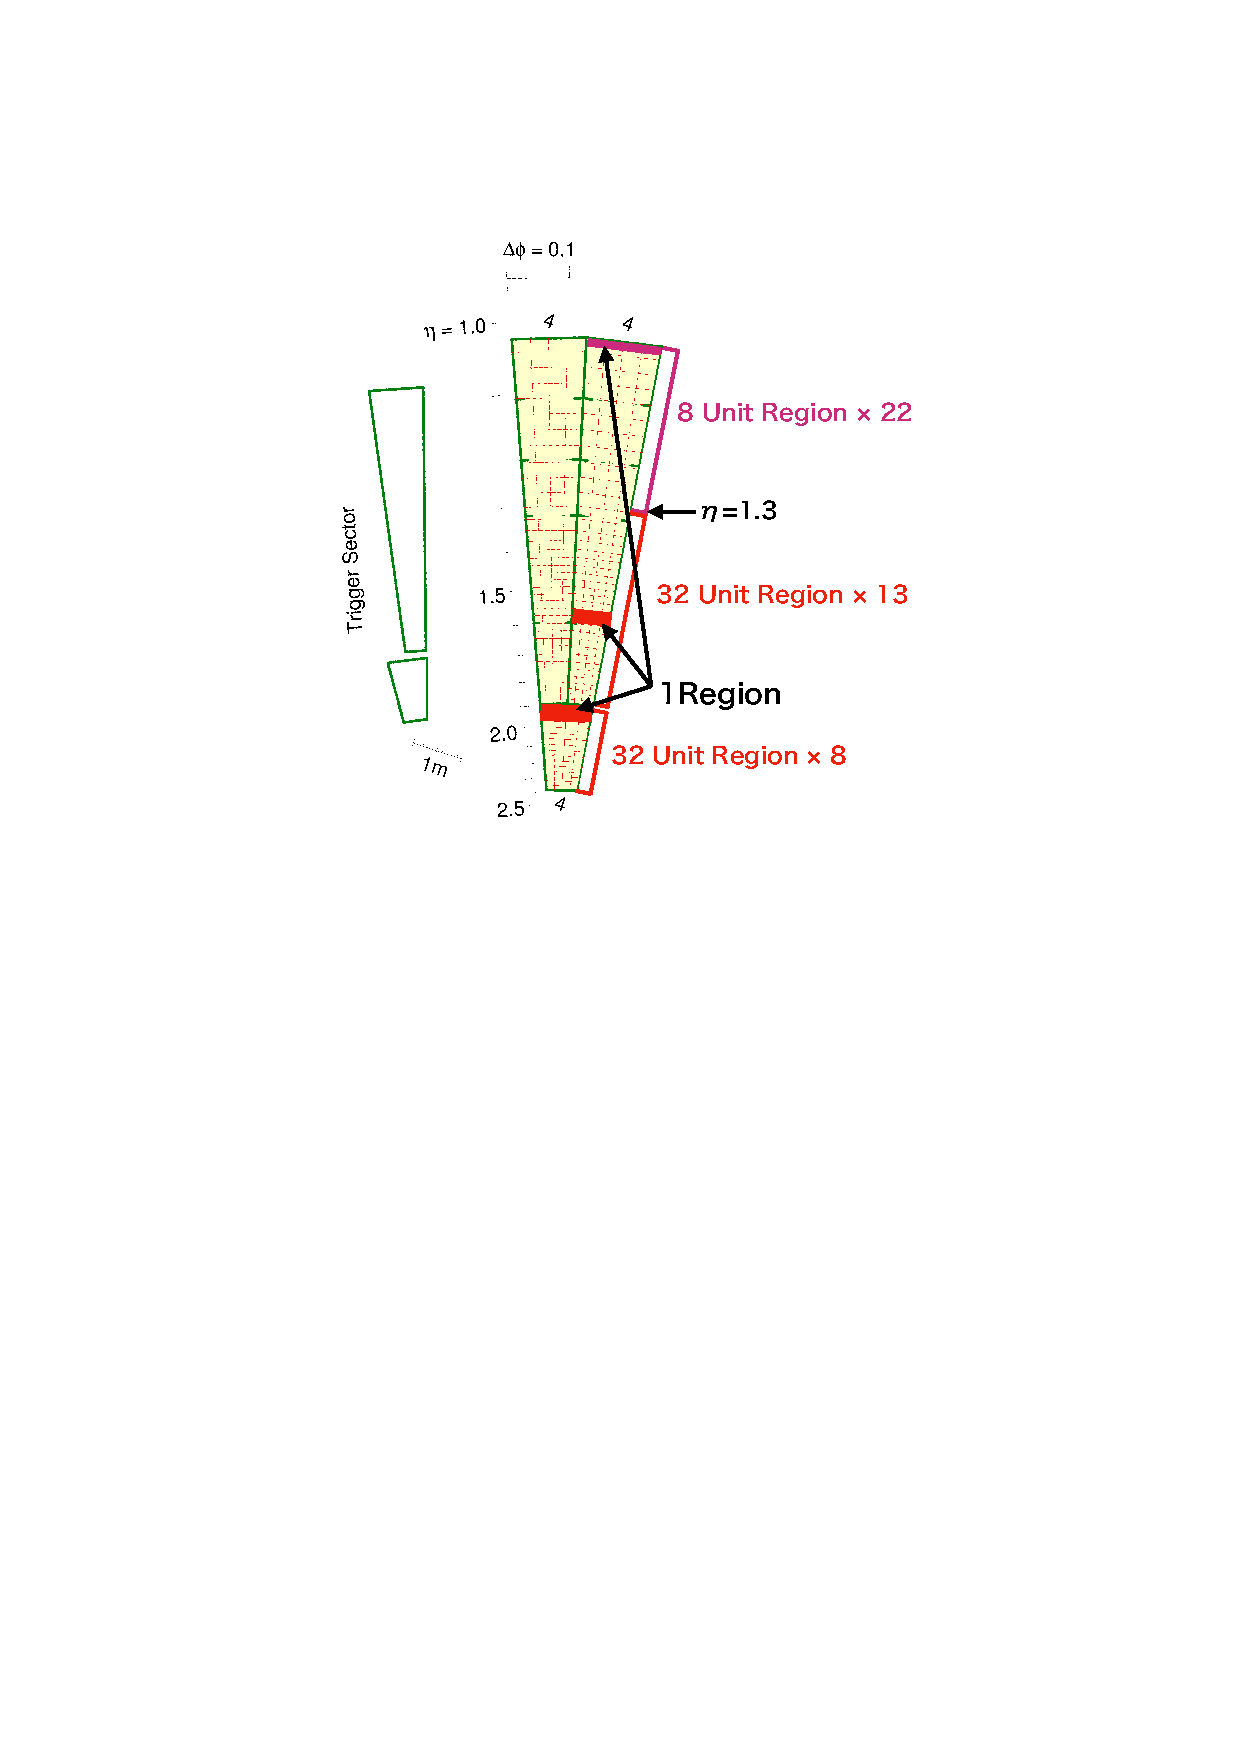
\includegraphics[width=12cm]{fig/SL/WS_region.pdf}
\caption[Wire Strip Coincidence以降のRegionの分割]{Wire Strip CoincidenceのRegionの定義\cite{mt_kawamoto}。エンドキャップ領域は|$\eta$| < 1.3 領域では 8 Unit、1.3 < |$\eta$| 領域では32 Unit という異なる大きさの Regionを定義し、それぞれの領域を22分割、13分割する。フォワード領域は32 Unit Regionで8分割する。
}
\label{WS_region}
\end{figure}

図\ref{WS_Concept}に1つのUnitの構造を示す。8 Unit Regionはトリガーセクターの全$\phi$領域に当たる、ストリップ4 Unitからのstrip segmentと ワイヤー2 Subunitからのwire segmentを組み合わせて、最大1つの飛跡候補を出力する。32 Unit Regionはストリップ 4 Unitからのstrip segmentと、ワイヤー 8 Subunitからのwire segmentを組み合わせて、最大4つの候補を出力する。SL全体では最大180の飛跡候補が出力される。

\begin{figure} 
\centering
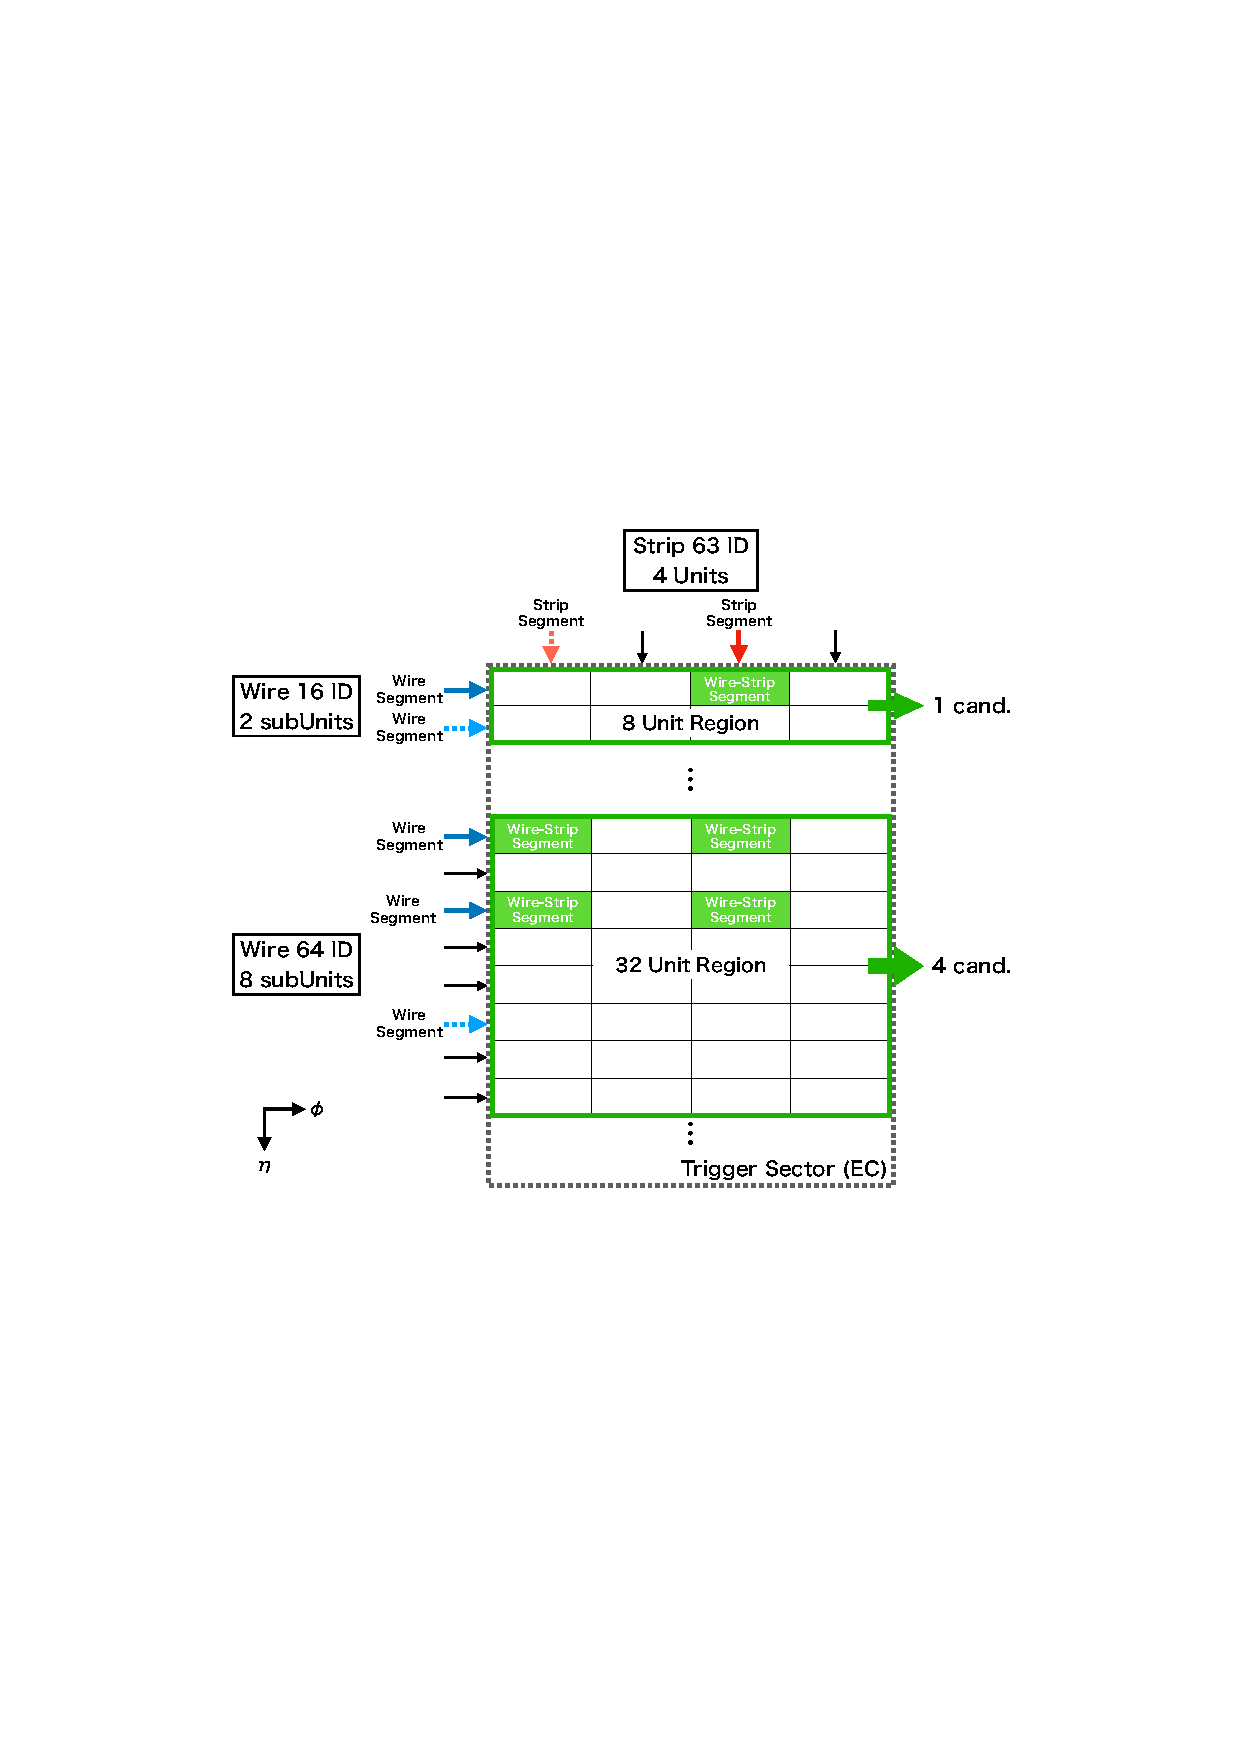
\includegraphics[width=16cm]{fig/SL/WS_Concept.pdf}
\caption[]{8 Unit Region、32 Unit Regionにおけるコインシデンスの概要\cite{mt_kawamoto}。8 Unit Regionではストリップ4 Unitからのstrip segmentと ワイヤー2 Subunitからのwire segmentの組み合わせから、最大1つの飛跡候補を出力する。32 Unit Regionはストリップ 4 Unitからのstrip segmentと、ワイヤー 8 Subunitからのwire segmentの組み合わせから、最大4つの候補を出力する。}
\label{WS_Concept}
\end{figure}

Wire Strip Coincidenceの各Unit内でのロジックの概要を図\ref{WS_logic}に示す。各ユニットは\pt  Calculator、Wire Position Corrector、Block Selectorで構成される。以下でそれぞれのモジュールについて説明する。

\begin{figure} 
\centering
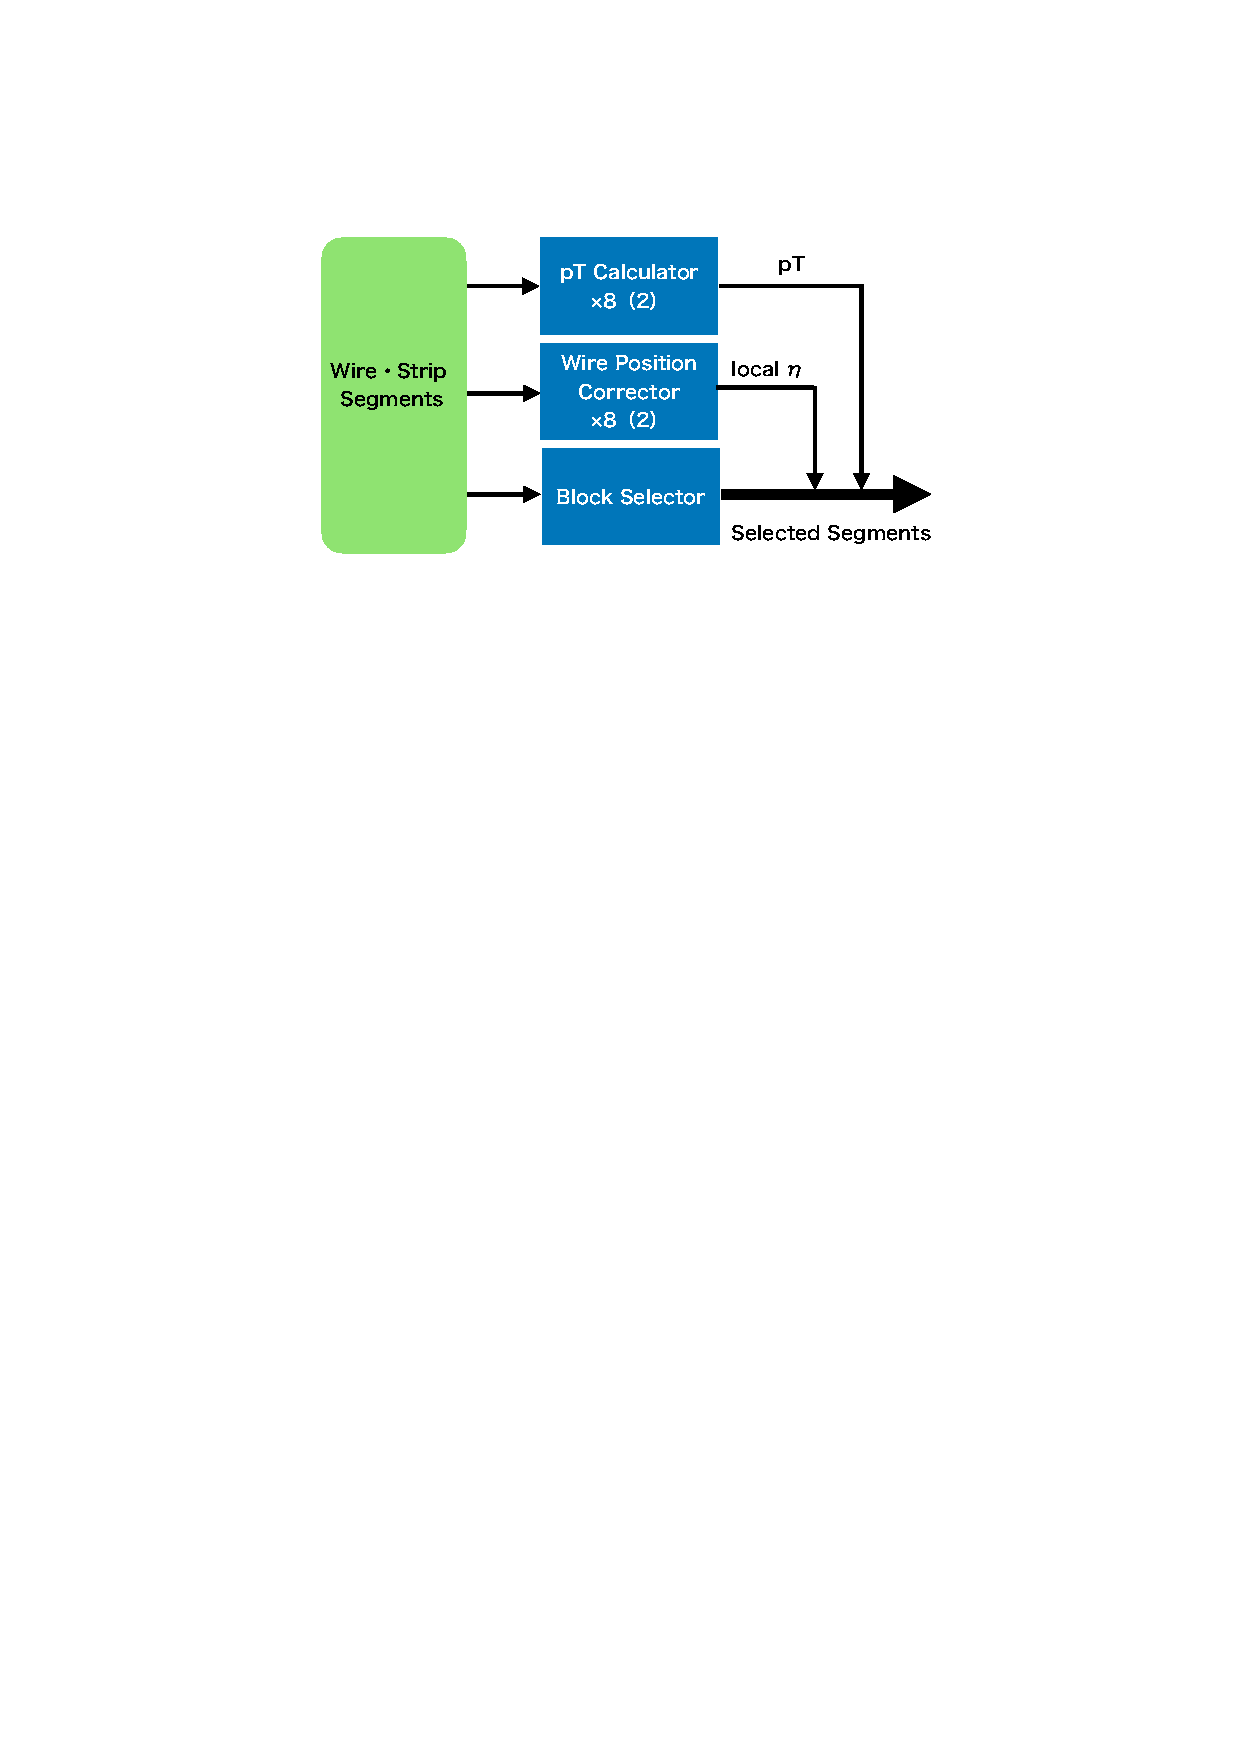
\includegraphics[width=16cm]{fig/SL/WS_logic.pdf}
\caption[Wire Strip Coincidence ファームウェアの概要]{Wire Strip Coincidence ファームウェアの概要\cite{mt_kawamoto}。Wire segmentおよびStrip Segmentの情報をもとに、$p_\mathrm{T}$を計算する$p_\mathrm{T}$ Calculator、localな$\eta$情報を計算するWire Position Corrector、複数のミューオン飛跡候補から後段に送信するものを選択するBlock Selectorで構成される。}
\label{WS_logic}
\end{figure}

\subsubsection*{\pt\,Calculator}
\pt\,Calculatorはwire segmentに含まれる8 bitの$\Delta\theta$及びstrip segmentに含まれる9 bitの$\Delta\phi$から、Coincidence Windowにアクセスするためのアドレスを作成し、Coincidence Windowに格納された4 bitの\pt を出力する。1つの\pt\,Calculatorは1つのwire segmentと4つのstrip segmentを組み合わせ、全ての組み合わせに対して\pt を出力する。Coincidence WindowはFPGAのdual BRAM上に格納されているため、この処理は160 MHzの2クロックチックで完了する。

\subsubsection*{Wire Position Corrector}
wire segment や strip segmentに含まれる位置情報は代表点番号だが、磁場内部の検出器からは主にヒットのあった$\eta$座標が送られる。そこでInner Coincidenceでは位置情報として$\eta$を統一的に用いる。しかし、TGC検出器における代表点番号と$\eta$の関係はUnit Regionごとにばらつきがあることが知られており\footnote{wireの代表点が$\eta$に対して均一に並んでいないことと、$\phi$位置ごとでも代表点と$\eta$の対応関係は異なることによる}、全てのUnitで共通に変換できる訳ではない。そこでwireとstripの代表点と$\eta$座標の対応関係をパターンリストとして保存し、Unitごとに$\eta$の再構成を行う。これを担当するモジュールをWire Position Correctorと呼ぶ。

\subsubsection*{Block Selector}
Block Selectorはワイヤーとストリップの組み合わせで生じる複数のミューオン飛跡候補から、後段に送る飛跡候補を選択する。飛跡の選抜はマッチした層数の多さを基準に行い、マッチした層数も同じ場合は角度がより小さいものを選択する。8 Unit Regionでは4つのストリップ飛跡と2つのワイヤー飛跡から再構成される計8個の飛跡候補から、最大1つの候補を絞り込む。32 Unit Regionでは4つのストリップ飛跡と8つのワイヤー飛跡の組み合わせからなる32個の飛跡候補から最大4つの候補を選ぶ。この時、2つは$\Delta\theta$が正の方向に曲げられたもの、もう2つは負に曲げられたものが選ばれるように設計する。これはJ/$\psi$ 粒子などから生じる、2つの異符号ミューオンを優先的に取れるようにするための実装である。
Wire Strip CoincidenceからInner Coincidenceに送られる飛跡情報のフォーマットを図\ref{tab:WS}に示す。

\begin{table}[]
    \centering
    \caption{Wire Strip Coincidenceにおける飛跡候補のデータフォーマット}
    \label{tab:WS}
    \begin{tabular}{|c|c|}
    \hline
    \# of bits & Name                                                                                        \\ \hline\hline
    1          & Valid flag which means this region receive the more than one strip segment and wire segment \\ \hline
    4          & $p_{\mathrm{T}}$ threshold reconstructed using Coincidence Window                           \\ \hline
    8          & Local $\eta$ position in the unit                                                           \\ \hline
    3          & Unit ID                                                                                     \\ \hline
    7          & Angle difference $\Delta\theta$ between the segment and the vector from IP                    \\ \hline
    2          & Number of stations with the hits used for wire segment reconstruction                       \\ \hline
    4          & Angle difference $\Delta\phi$ between the segment and the vector from IP                    \\ \hline
    2          & Number of stations with the hits used for strip segment reconstruction                      \\ \hline
    \end{tabular}
\end{table}

\subsection{Inner Coincidence}
\subsubsection*{概要}
Inner CoincidenceではTGC BW コインシデンスで再構成された飛跡候補と磁場領域内部の検出器 (NSW、RPC BIS78、TGC EI、Tile カロリメーター)でコインシデンスととることで、衝突点に由来しないフェイクトリガーの削減と\pt 分解能の向上を図る。図\ref{SL_InnerCoin_covarage}に各検出器がカバーする$\eta$、$\phi$領域を示す。1.3 < $\eta$ < 2.4の領域はNSWが網羅的にカバーしており、1.05 < $\eta$ < 1.3領域ではTGC EI、RPC BIS78、Tile カロリメーターがそれぞれ相補的にカバーしている。
\begin{figure} 
    \centering
    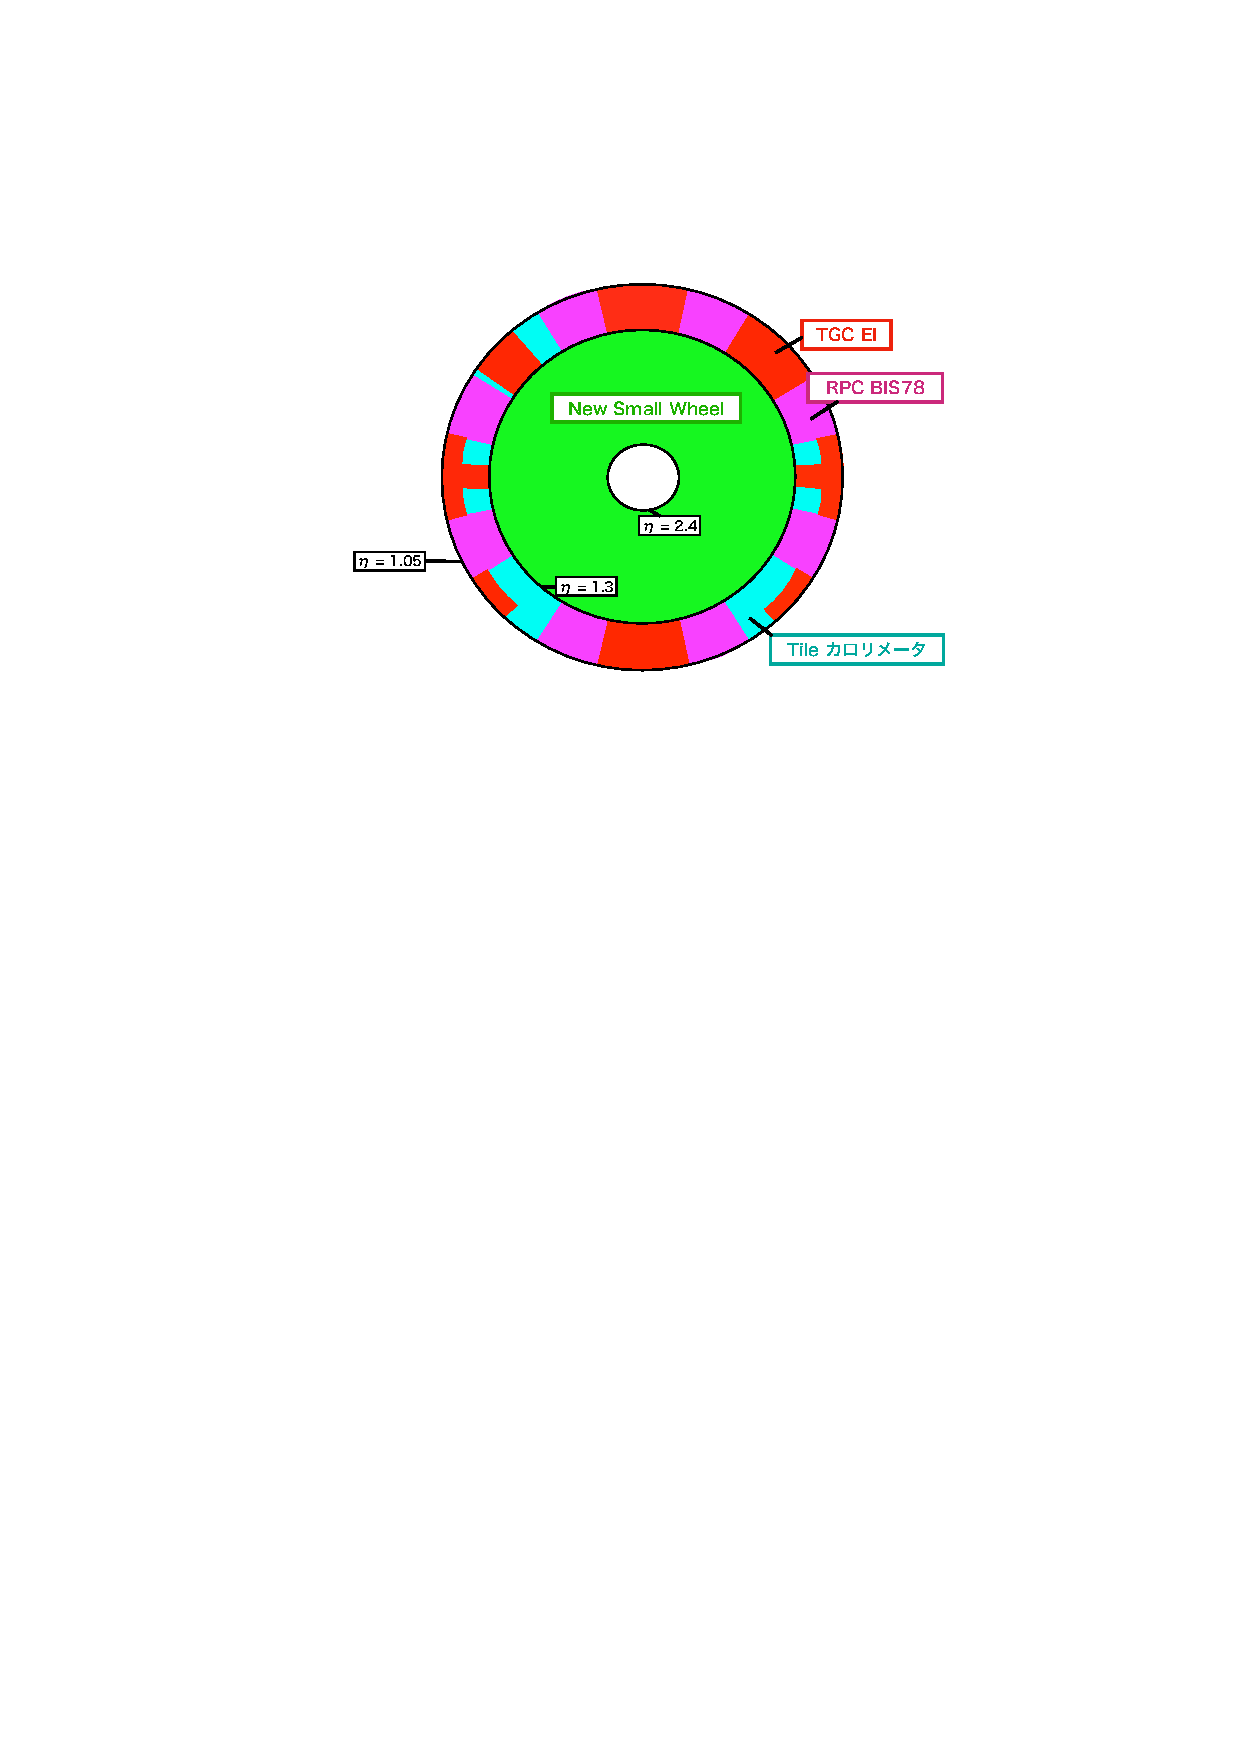
\includegraphics[width=16cm]{fig/Intro/SL_InnerCoin_covarage.pdf}
    \caption[磁場内部の検出器でカバーされる$\eta$、$\phi$領域]{各磁場内部の検出器がカバーする$\eta$、$\phi$領域\cite{mt_mino}。|$\eta$| < 1.3 領域はNSWがカバーする。1.3 < |$\eta$| 領域はTGC EI、RPC BIS 78、Tile カロリメーターがそれぞれ相補的にカバーしている。}
    \label{SL_InnerCoin_covarage}
\end{figure}

磁場内部に位置する検出器はそれぞれ異なる特徴を持っているため、コインシデンスをとる検出器ごとに独立したロジックが用意されている。ここでは具体例としてNSWとのコインシデンスロジックについて説明する。

図\ref{Concept_NSW}にNSWとのコインシデンスアルゴリズムの概要を示す。衝突点から飛来するミューオンはNSWにヒットを残した後エンドキャップトロイド磁場により主に$\eta$方向に曲げられ、TGCにヒットを残す。そのためTGC BW Coincidence で再構成された$\eta$位置($\eta_{\mathrm{TGC}}$)とNSWで再構成された$\eta$位置($\eta_{\mathrm{NSW}}$)の差は\pt と相関をもつ。この差を$d\eta$とよぶ。

\begin{figure} 
\centering
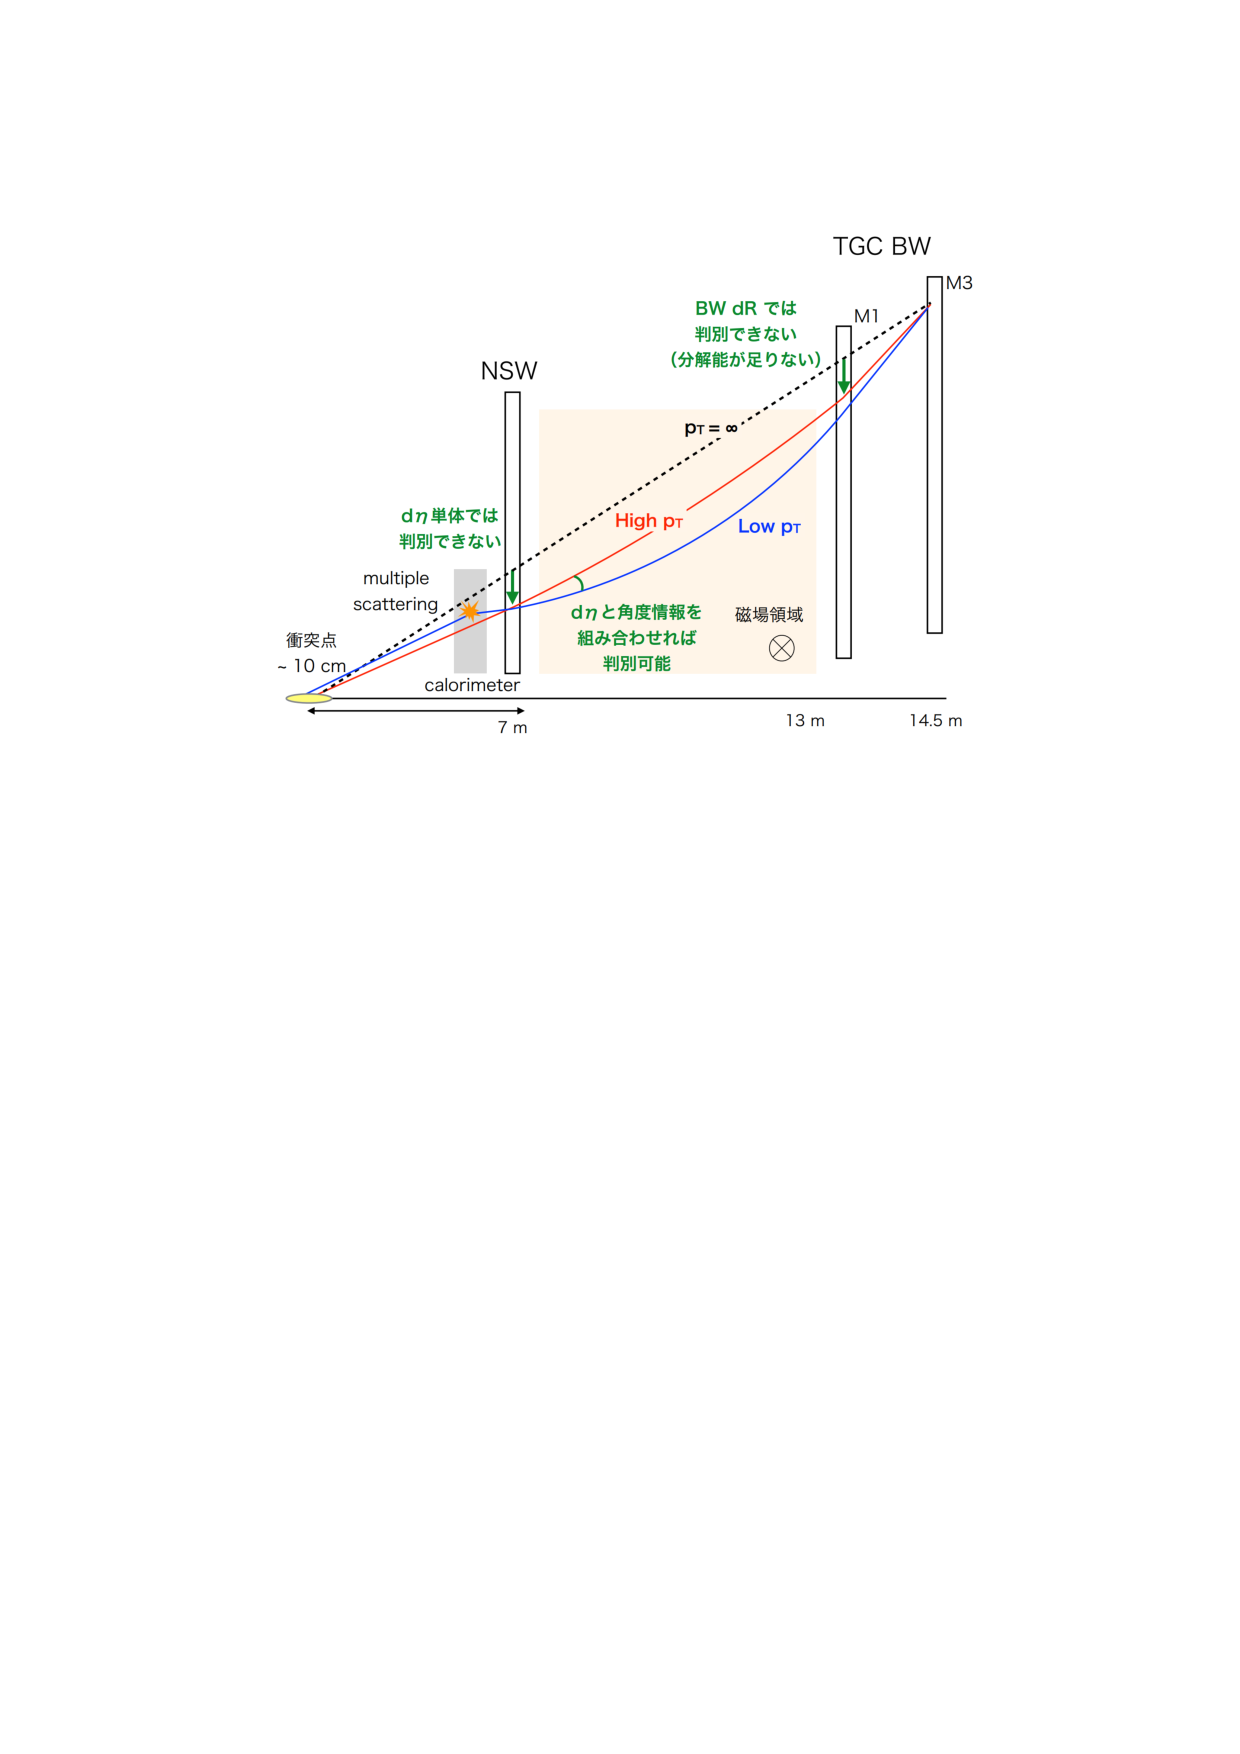
\includegraphics[width=16cm]{fig/SL/Concept_NSW.pdf}
\caption[NSW を用いたコインシデンスロジックの概要]{NSW を用いたコインシデンスロジックの概要\cite{mt_akatsuka}。$p_\mathrm{T}$が小さいミューオンほど磁場領域で曲げられるため、基本的には$d\eta$を用いることで$p_\mathrm{T}$を判定することができる。しかし、青線で示すようにNSWに入射する前に多重散乱を受けた場合には、$d\eta$だけではHigh $p_\mathrm{T}$のミューオンとLow $p_\mathrm{T}$のミューオンを判別することができない。そこでNSWに入射した角度 ($\Delta\theta_{\mathrm{NSW}}$) を分別変数として追加することで、より正確に$p_\mathrm{T}$ を判定することができる。}
\label{Concept_NSW}
\end{figure}

\begin{equation}
    d\eta = \eta_{\mathrm{TGC}} - \eta_{\mathrm{NSW}}
    \label{eq:deta}
\end{equation}

一方、衝突点から飛来するミューオンは検出器内部の物質 ( 主に物質量の大きいカロリーメータ )と多重散乱を起こすことがあり、この場合では$d\eta$のみでは\pt が高いものと低いものを見分けることができない。そこで、ミューオンがNSWに入射した角度 ($\Delta\theta_{\mathrm{NSW}}$) を分別変数として追加することで、より正確に\pt 判定を行うことができる。この計算には$d\eta$、$\Delta\theta_{\mathrm{NSW}}$ を入力、\pt を出力としたCoincidence Windowを利用する。

\subsubsection*{Inner Coincidenceの論理回路実装}
このモジュールの駆動クロックは、LHC クロックに同期した周波数 160 MHz のクロックで、レイテンシーは 7 クロックチック分 (43.75 ns) である。
Inner CoincidenceもRegionを1単位として並列に処理が行われる。$\eta$位置ごとにどの検出器とコインシデンスをとるかが決められており、|$\eta$| < 1.3 の領域では主にRPC、EI、Tileカロリメーターと、|$\eta$| > 1.3の領域では主にNSWとコインシデンスをとる。8 Unit RegionはWire Strip Coincidenceから1つの飛跡候補を受け取り、磁場内部の検出器とコインシデンスをとった後、1候補を出力する。32 Unit RegionはWire Strip Coincidenceから4つの飛跡候補を受け取り、2つまで候補を絞って出力する。その結果SL全体では最大112候補を出力する。

Inner Coincidenceの各Unit 内でのロジックの概要を図\ref{Inner_logic}に示す。各ユニットはDecoder、Coincidence、Which Innerで構成される。以下に例としてNSWとのコインシデンスをとるRegionについて説明する。

\begin{figure} 
\centering
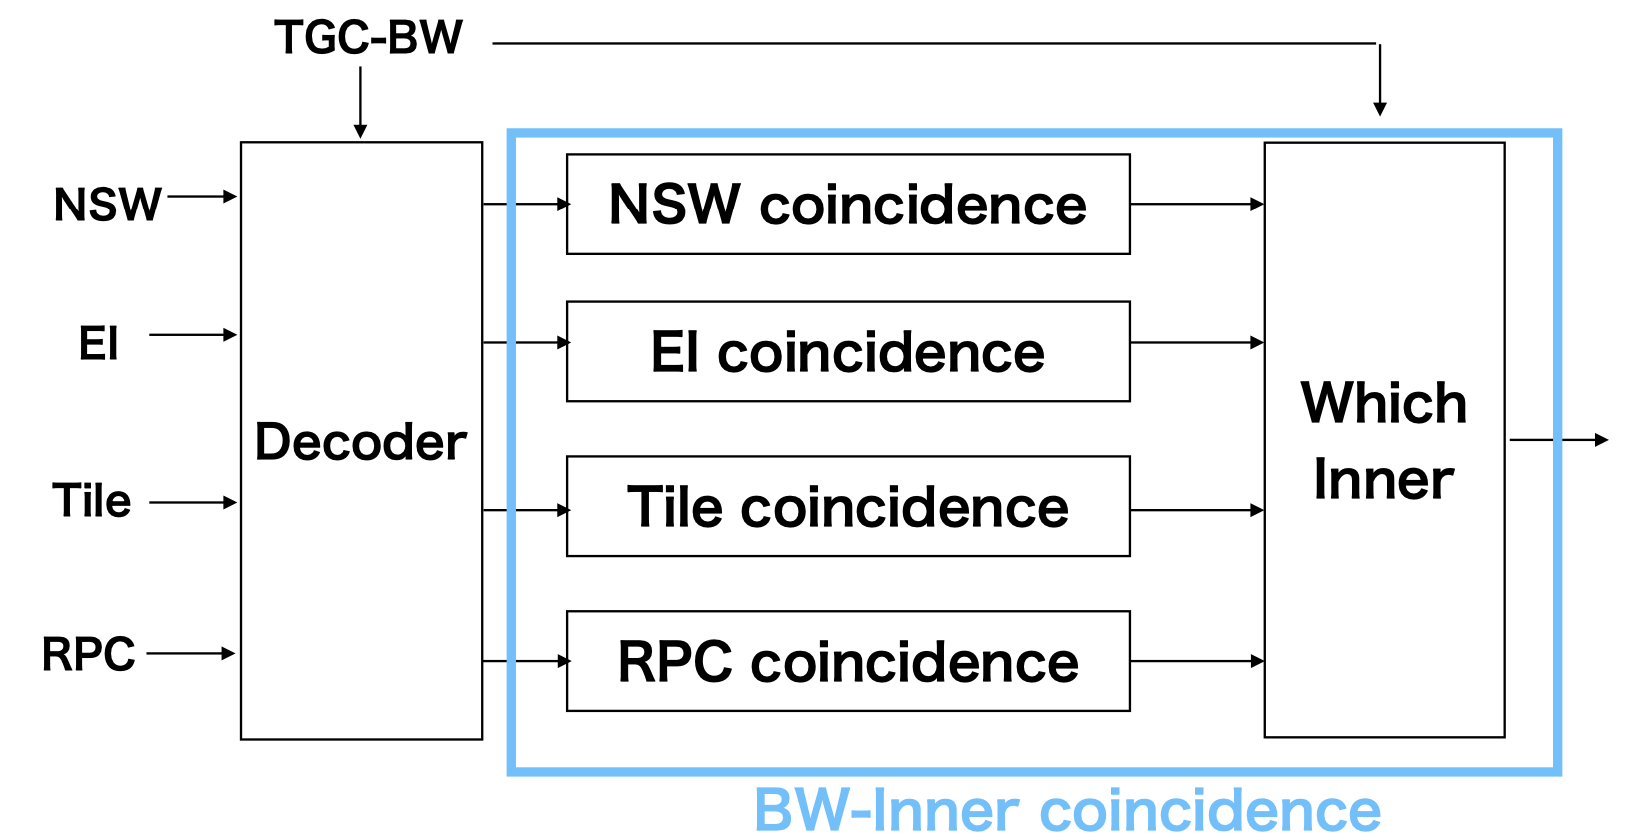
\includegraphics[width=16cm]{fig/SL/Inner_integrate.png}
\caption[Inner Coincidenceの概要]{Inner Coincidenceの概要\cite{mt_kobayashi}。Inner CoincidenceはNSWから受け取った飛跡候補のうち、コインシデンスに利用する候補を選ぶDecoder、各検出器とのコインシデンスロジック、どの検出器とのコインシデンス結果を採用するか選択するWhich Inner で構成される。}
\label{Inner_logic}
\end{figure}

\begin{itemize}
    \item Decoder\\
    1つのSLはNSWで再構成された飛跡を最大16個受け取る。この中からTGC BW コインシデンスで再構成された飛跡候補と組み合わせる4候補を選ぶのがDecoderである。ここでは \pt が大きいミューオンの検出効率を高く保つため、|$d\eta$| が小さいものを優先的に選別する。
    \item NSW Coincidence\\
    TGC BW の1つの飛跡候補とNSWの4つの飛跡候補でコインシデンスをとる。Coincidence WindowはFPGAのURAMに格納されており、8 bitの$d\eta$情報と4 bitの$\Delta\theta$を入力、4 bitの\pt を出力とする。計算された飛跡のうち、\pt が最大の候補が保存され40 MHzごとに出力される。
    \item Which Inner\\
    Which Inner モジュールは複数の検出器とのコインシデンスロジックが並列に走る|$\eta$| < 1.3の領域において、どの検出器とのコインシデンス結果を最終出力とするかを決定する。
\end{itemize}
Inner CoincidenceからTrack Selectorに送られる飛跡候補のデータフォーマットを表 \ref{tab:InnerCoin} に示す。

\begin{table}[]
    \centering
    \caption{Inner Coincidenceにおける飛跡候補のデータフォーマット}
    \label{tab:InnerCoin}
    \begin{tabular}{|c|c|c|}
    \hline
    \# of bits & Name                             & Comment                                                                \\ \hline\hline
    14         & TGC $\eta$                       & $\eta$ in global candidate at the pivot plane of TGC                   \\ \hline
    9          & TGC $\phi$                       & $\phi$ in global candidate at the pivot plane of TGC                   \\ \hline
    8          & TGC $p_\mathrm{T}$               & TGC transverse momentum                                                \\ \hline
    4          & TGC $p_\mathrm{T}$ threshold     & TGChighest $p_\mathrm{T}$     threshold satisfied                       \\ \hline
    1          & TGC charge                       & TGC TC charge                                                          \\ \hline
    3          & Coincidence type                 & Identifier of coincidence type                                         \\ \hline
    14         & MDT $\eta$                       & $\eta$ coordinate of the MDT segment position of the innermost station \\ \hline
    8          & MDT $p_\mathrm{T}$               & MDT transverse momentum                                                \\ \hline
    4          & MDT $p_\mathrm{T}$ threshold     & MDT highest transverse momentum threshold satisfied                         \\ \hline
    1          & MDT charge                       & MDT charge                                                             \\ \hline
    4          & MDT Processing Flag              & Type of reconstructed muon                                             \\ \hline
    2          & \# of segments                   & Number of MDT segments associated to the muon                          \\ \hline
    3          & Segment quality flag             & Quality of each segment                                                \\ \hline
    49         & Reserved                         &                                                                        \\ \hline
    \end{tabular}
\end{table}

\subsection{Track Selector}
\subsubsection*{概要}
Track SelectorはInner Coincidenceから出力される最大112個のミューオン飛跡候補からMUCTPIに送る6候補を選ぶ。このときInner Coincidenceで判定された\pt が高いものを優先的に選択する。

\subsubsection*{Track Selectorの論理回路実装}
モジュールの駆動クロックはLHCクロックに同期した周波数160 MHzのクロックで、レイテンシーは 5 クロックチック (31.25 ns) である。
概要を図\ref{TrackSelector_overview}に示す。Track Selectorは112個のミューオン飛跡候補を\pt が大きい順に並び替えるソーティングロジックとして実装される。特にBatcherの奇遇マージソート法\cite{Batcher}という、高速かつ並列にソーティングを行うメソッドをデジタル回路として実現している。Track Selectorは16個の8-key sorting network、と15個の16-key merging networkで構成され、インプットが128、アウトプットが8のソーティングロジックとなっている。8-key sorting networkおよび16-key merging networkの概要を図\ref{Sortiing_8key}、\ref{Sorting_16}に示す。これらの図の横線はワイヤーを示し、縦線がコンパレーターを表す。左から右に1つの飛跡候補同士の比較が行われ、それの集合体としてロジックが実装される。


\begin{figure} 
    \centering
    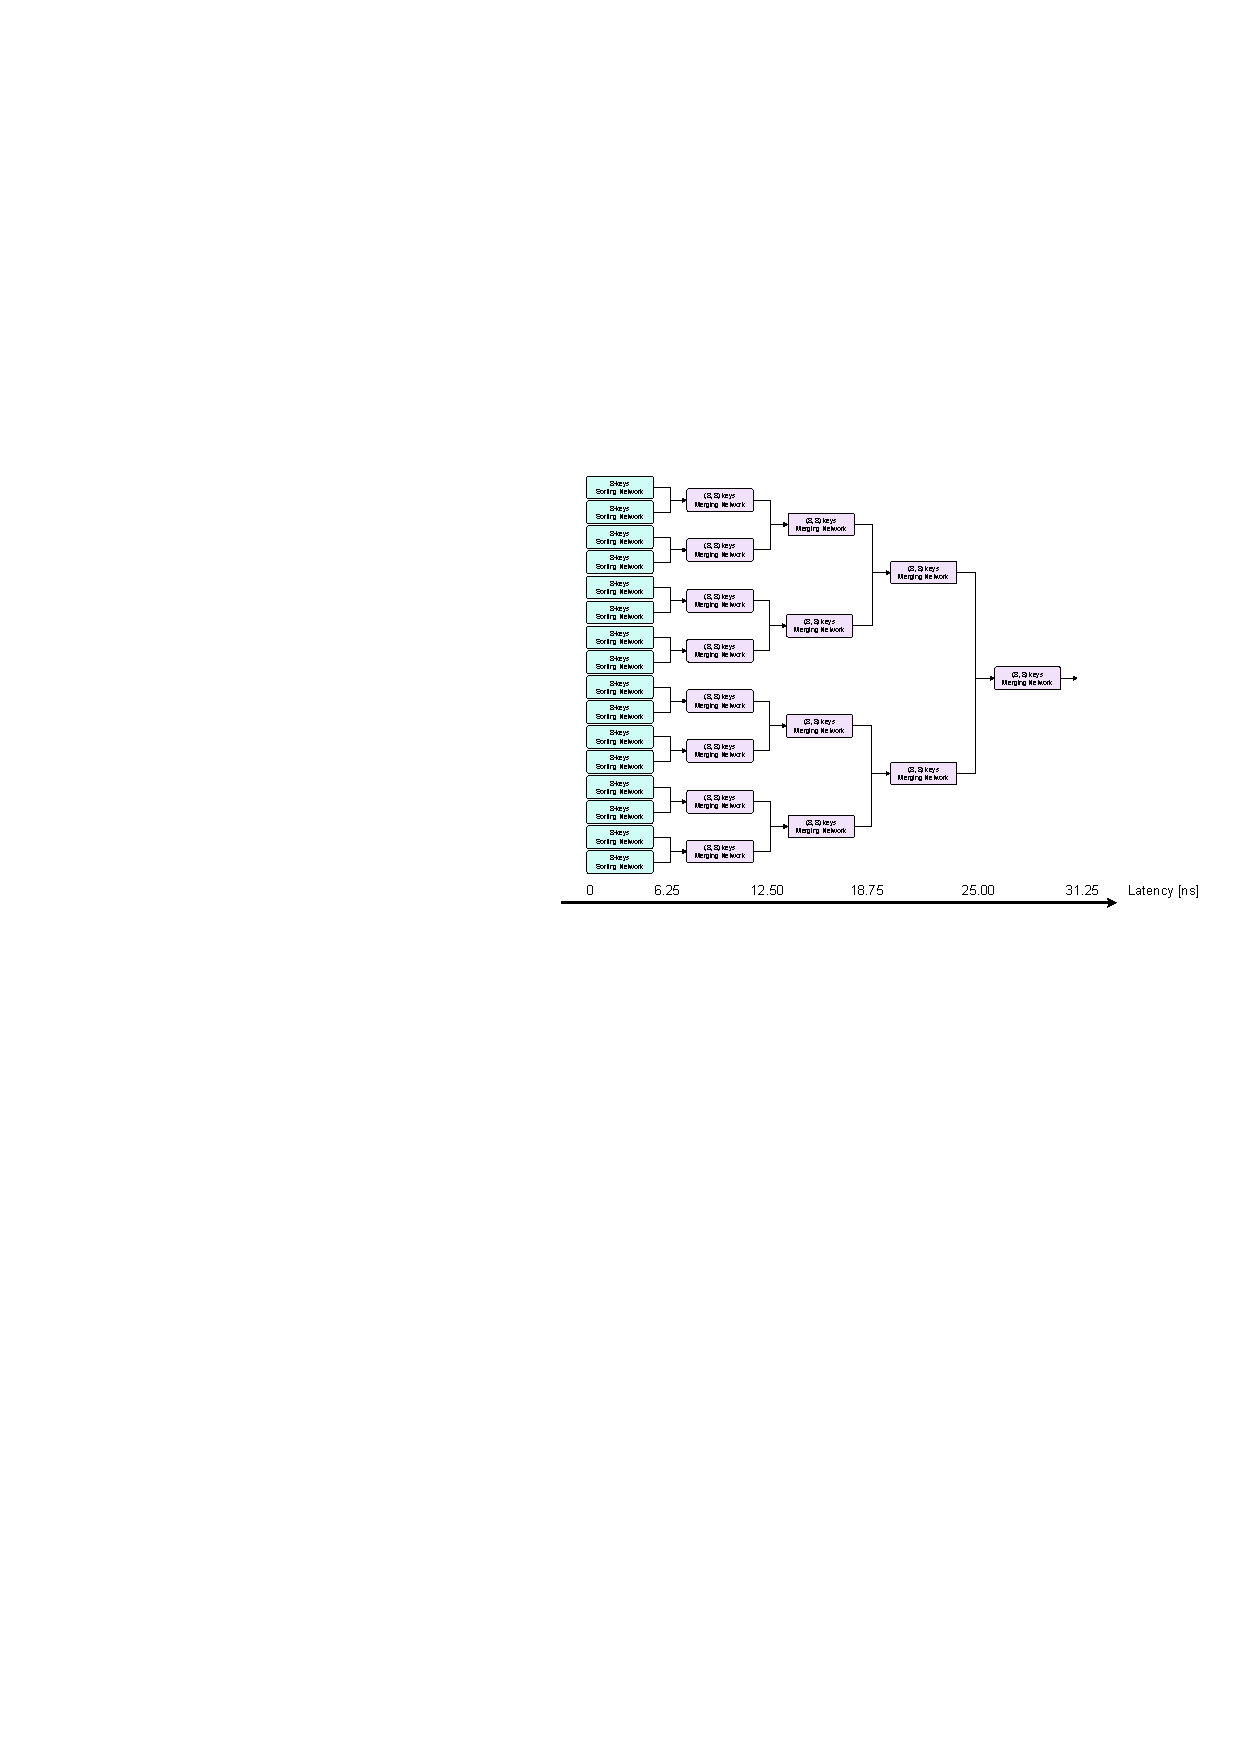
\includegraphics[width=16cm]{fig/SL/TrackSelector_overview.pdf}
    \caption[Track Selector の概要]{Track Selector の概要。16個の8-key sorting network、と15個の16-key merging networkを用いて、128個のミューオン候補から$p_\mathrm{T}$が大きい順に8候補を選択する。このうち6個をMUCTPIに送信する。}
    \label{TrackSelector_overview}  
\end{figure}
    

\begin{figure} 
\centering
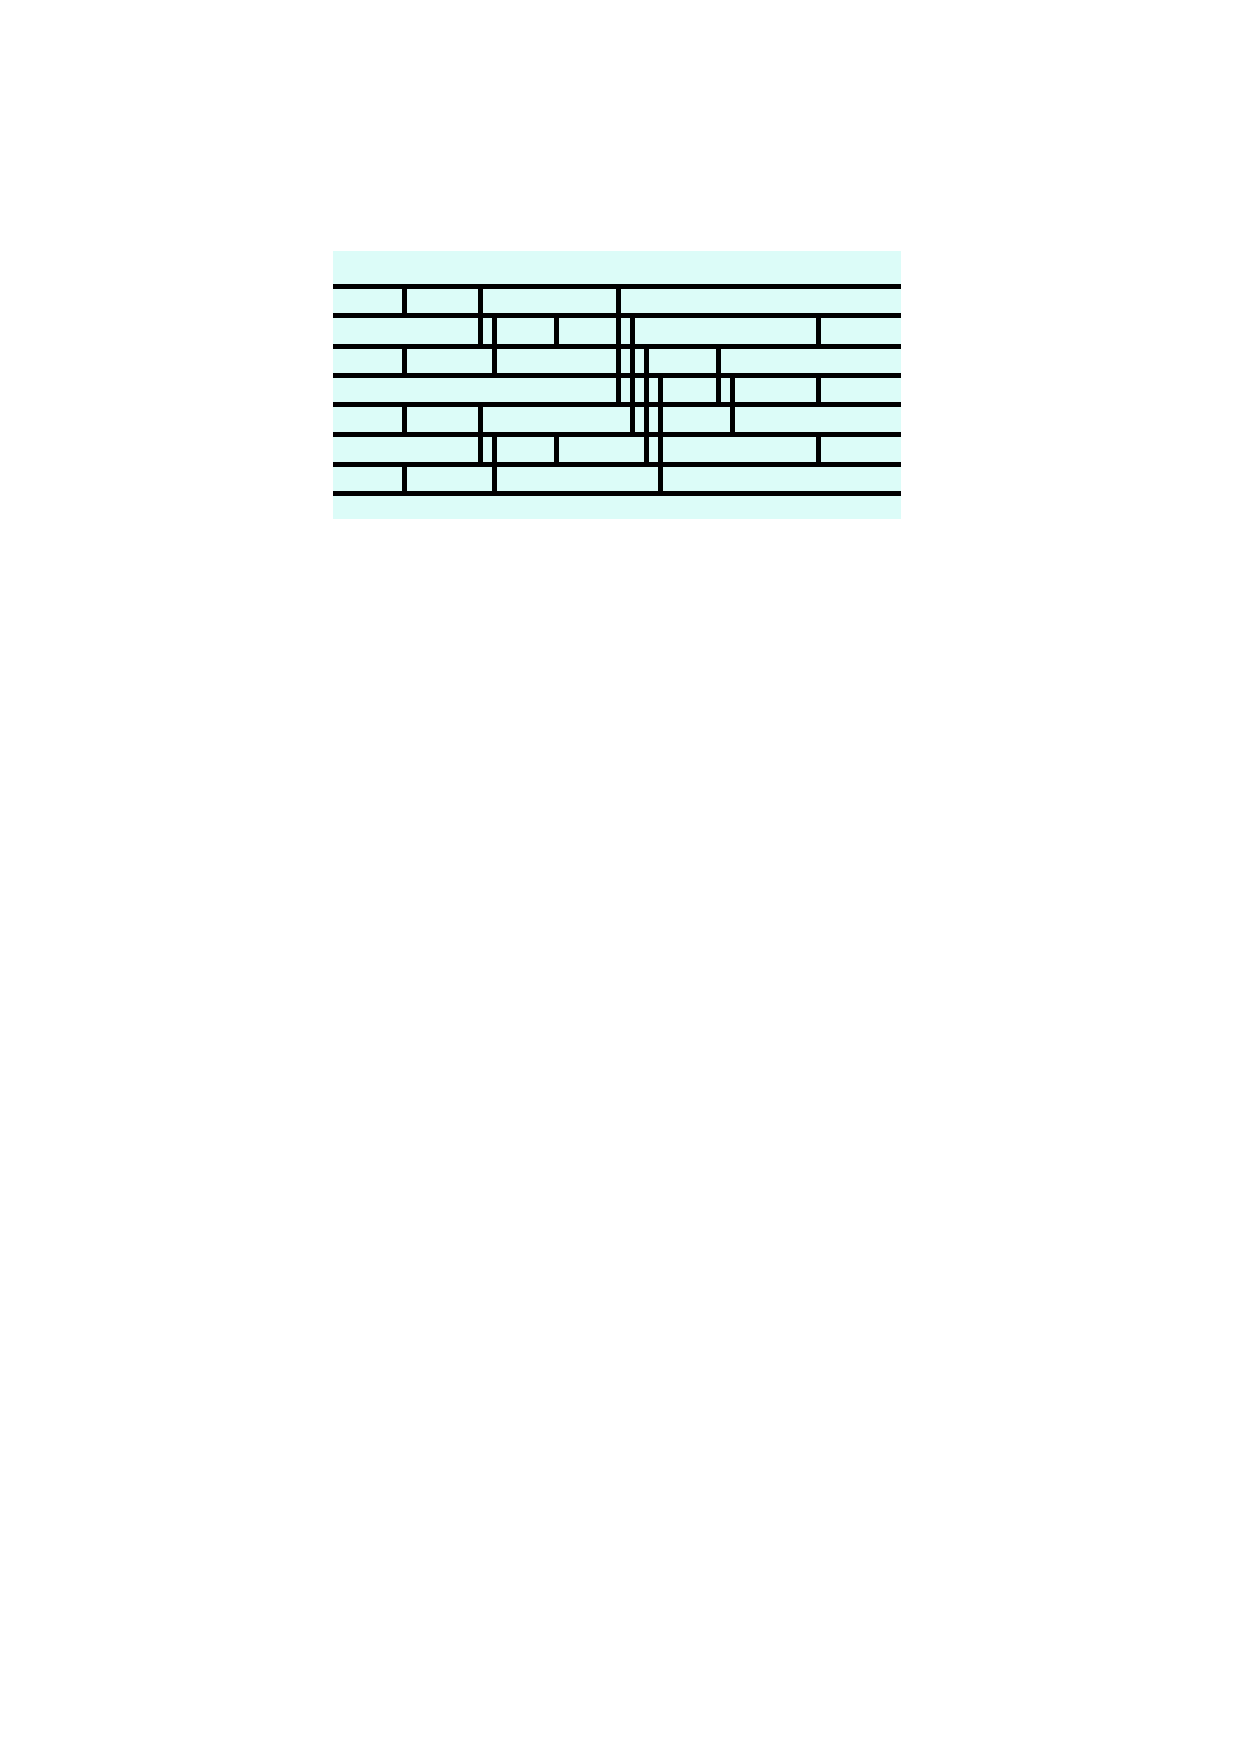
\includegraphics[width=10cm]{fig/SL/Sortiing_8key.pdf}
\caption[8-key sorting network の概要]{8-key sorting network の概要。横線はワイヤーを表し、縦線はコンパレーターを表す。}
\label{Sortiing_8key}
\end{figure}

\begin{figure} 
\centering
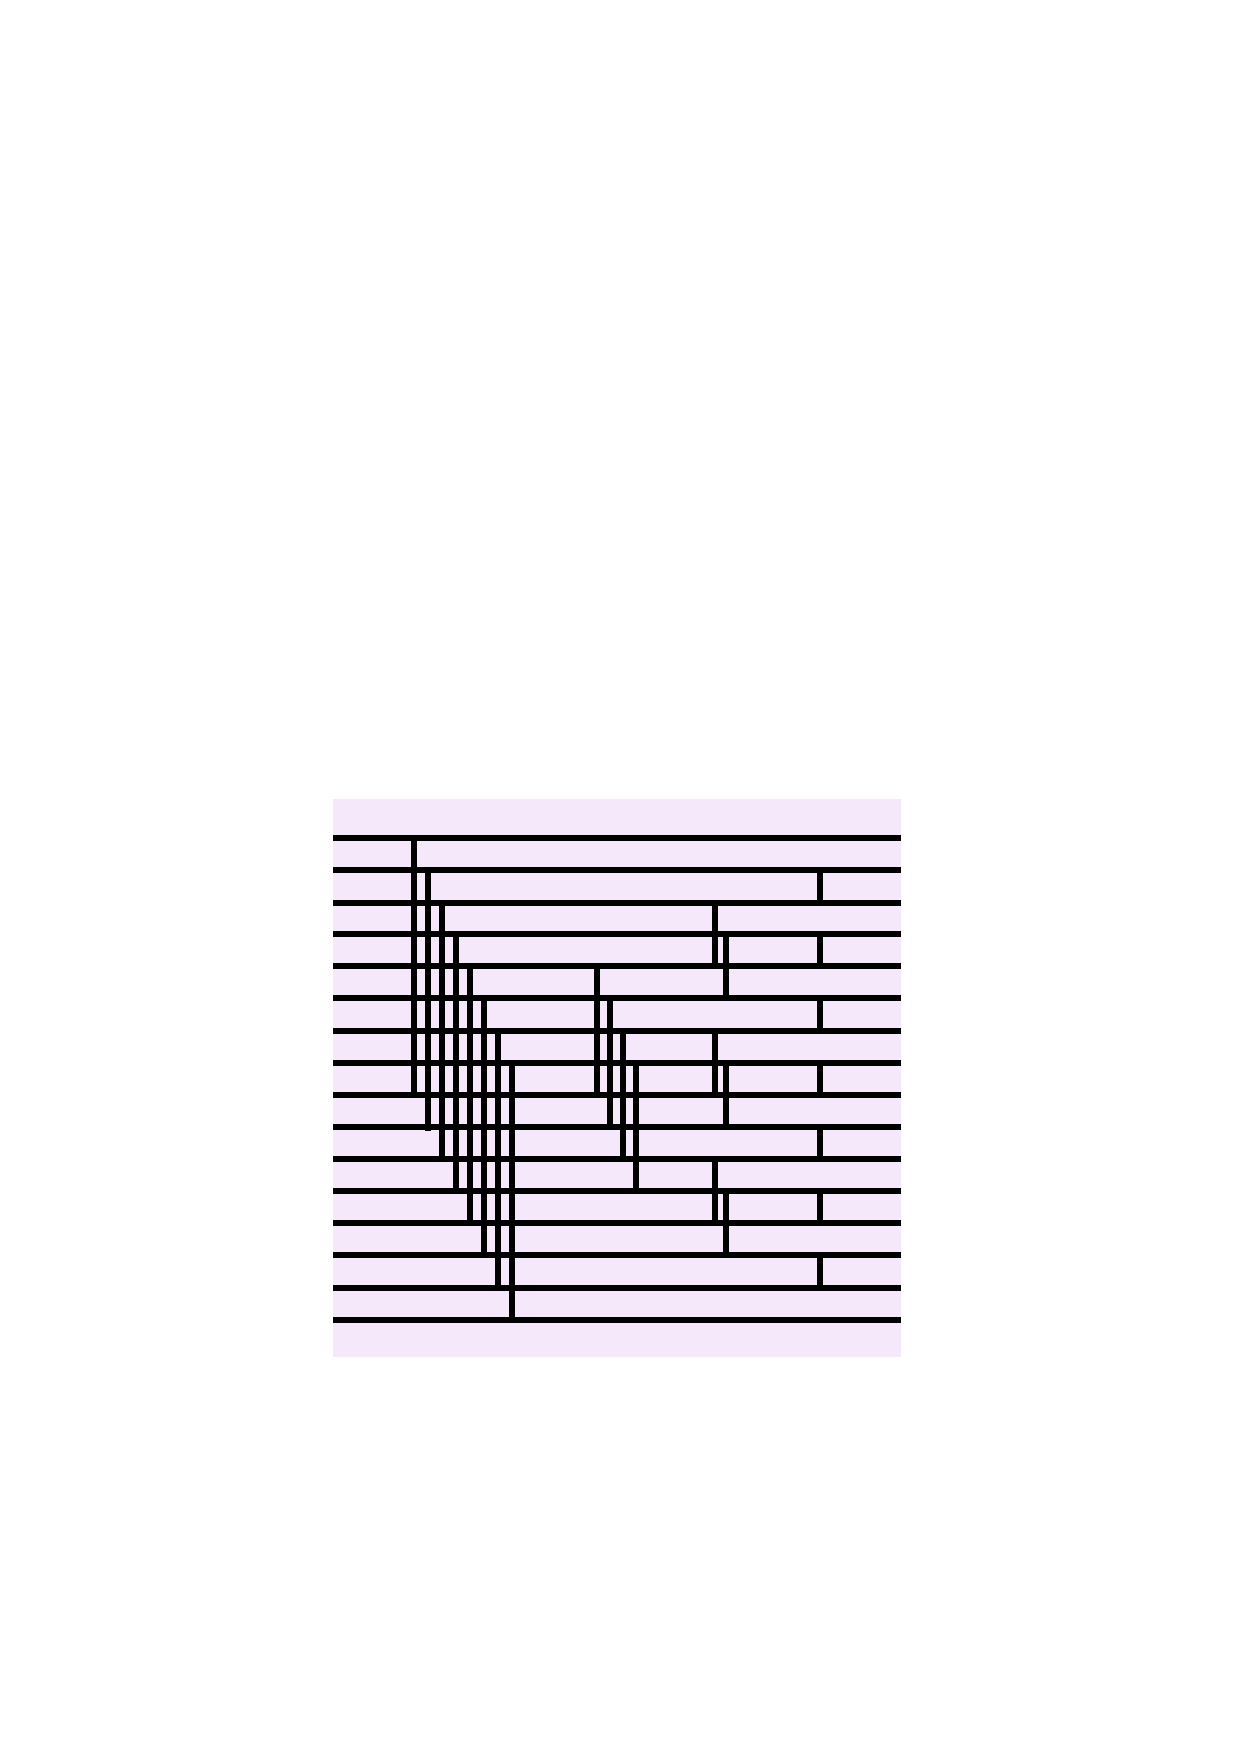
\includegraphics[width=10cm]{fig/SL/Sorting_16.pdf}
\caption[16-key merging network の概要]{16-key merging network の概要。横線はワイヤーを表し、縦線はコンパレーターを表す。}
\label{Sorting_16}
\end{figure}

\section{トリガーロジックの統合}
\label{sec_TriggerIntegration}
2章で述べたように、SL FPGAは4つのシリコンダイで構成されており、トリガーロジックはそれぞれのSLR上に並列に配置される(図\ref{Trigger_floor})。
PS board とのインターフェイスが実装されるSLR0・2・3には、TGC BW Coincidenceが実装される。トリガーセクターごとにSLRが分けられ、SLR0にEndcap $\phi\,0$、SLR2にEndcap $\phi\,1$、SLR3にForwardのロジックが配置される。磁場内部の検出器やMUCTPI、MDTTPとのインターフェイスはSLR1に実装され、ここにはInner Coincidence、Track Selectorが配置される。

\begin{figure} 
\centering
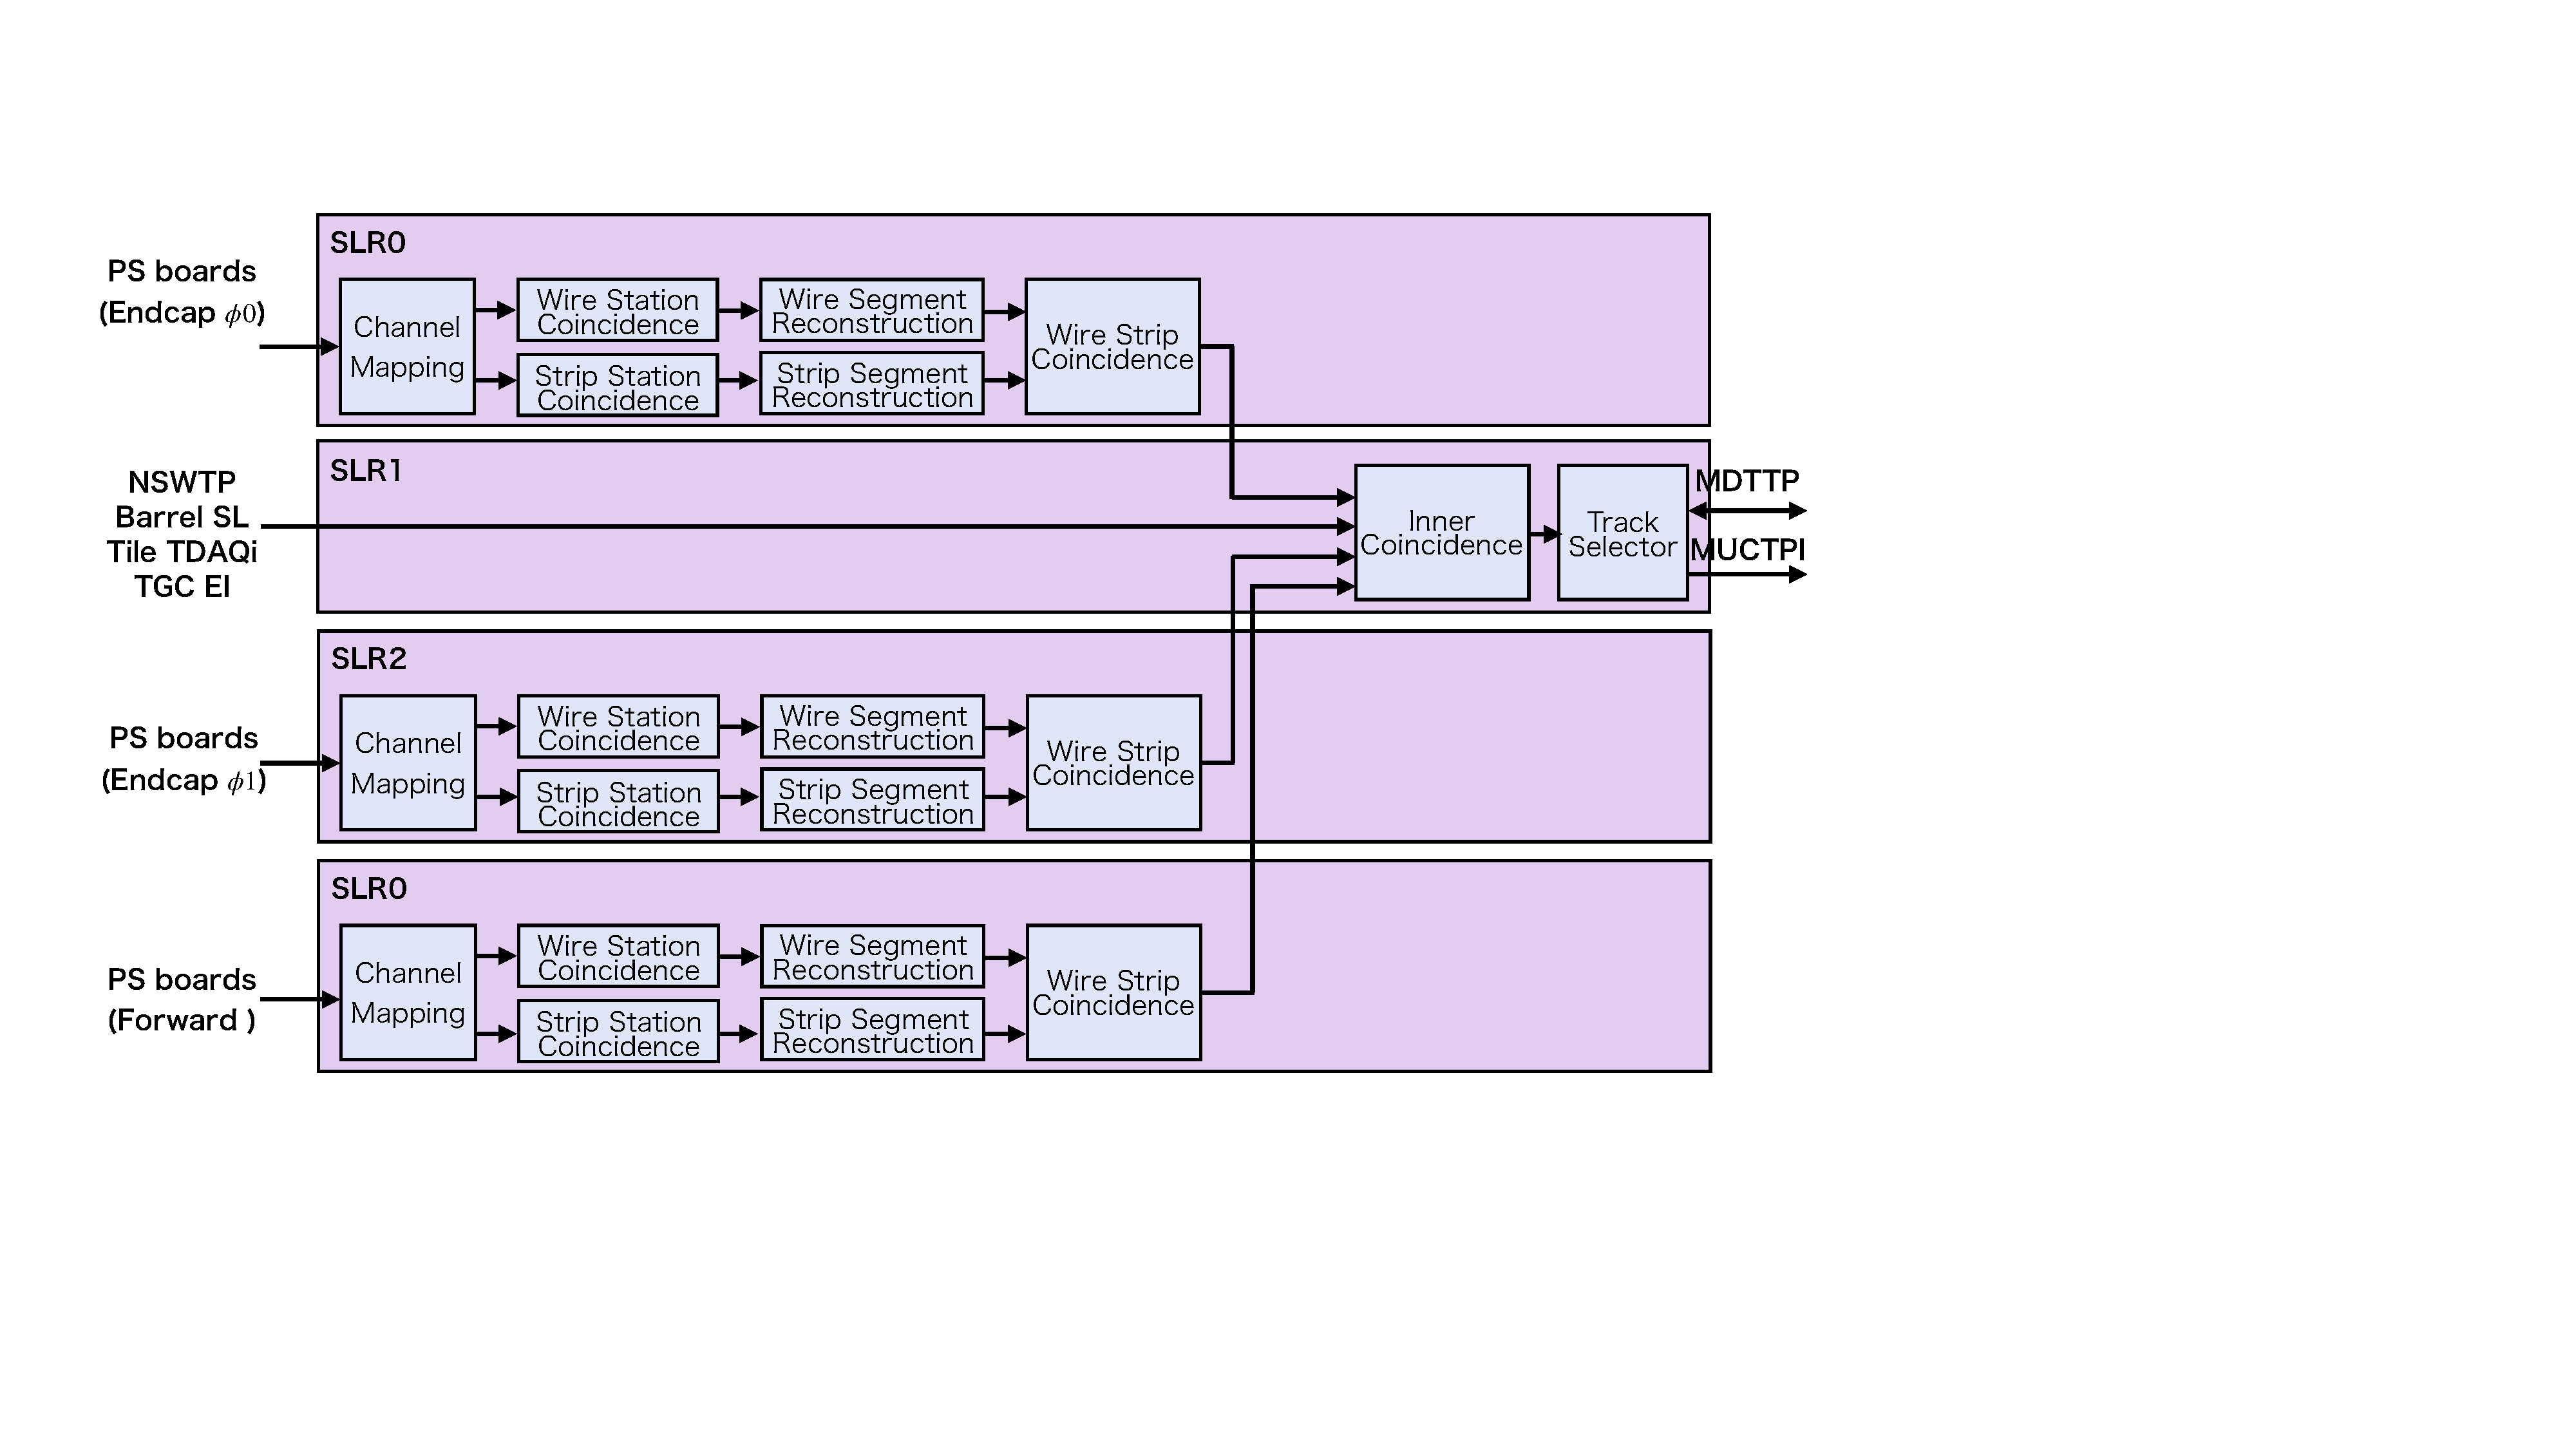
\includegraphics[width=16cm]{fig/SL/Trigger_floor.pdf}
\caption[SL FPGA内におけるトリガーロジックの配置]{SL FPGA内におけるトリガーロジックの配置。PS board とのインターフェイスが実装されるSLR0・2・3には、TGC BW Coincidenceが実装される。トリガーセクターごとにSLRが分けられ、SLR0にEndcap $\phi\,0$、SLR2にEndcap $\phi\,1$、SLR3にForwardのロジックが配置される。磁場内部の検出器やMUCTPI、MDTTPとのインターフェイスはSLR1に実装され、ここにはInner Coincidence、Track Selectorが配置される。}
\label{Trigger_floor}
\end{figure}

高輝度LHC-ATLAS実験に向けたトリガーロジックの開発は、これまでに各トリガーモジュールの論理回路実装が完了し、Segment Reconstructionまで全体ファームウェアへの統合が進められている。
本研究では引き続きWire Strip Coincidence、Inner Coincidence、Track Selectorの統合を進め、一連のトリガーロジックの統合を完了させる。以下にそれぞれの実装について述べる。

\subsection{Wire Strip Coincidenceの統合}
Wire Strip Coincidenceを統合ファームウェアに組み込むため、前段のWire Segment Reconstruction、Strip Segment Reconstructionの出力を配線した。また、モジュール内に存在する\pt  閾値概算用のLUTと$\eta$位置算出用のLUTをコンフィギュレーションするパスをそれぞれ接続した。
Wire Strip Coincidenceモジュールに接続した各信号線とそのバス幅について表\ref{tab:WS_integrate}にまとめる。

\begin{table}[]
    \centering
    \caption{Wire Strip Coincidenceにおける信号線}
    \label{tab:WS_integrate}
    \begin{tabular}{|c|c|}
    \hline
    接続するモジュール                               & 信号線 (バス幅 )                                                                                                    \\ \hline\hline
    Wire Segment Reconstruction             & \begin{tabular}[c]{@{}c@{}}Wire Segment ( EC : 148 subunit $\times$ 20 bit、 \\ FW : 64 subunit $\times$ 20 bit )\end{tabular} \\ \hline
    Strip Segment Reconstruction            & Strip Segment  ( EC : 20 unit   $\times$ 17 bit、FW : 5 unit $\times$ 17 bit)                                                    \\ \hline
    LUT Manager for $p_\mathrm{T}$ LUT      & Address + Data ( EC : 35 region $\times$ 18 bit、FW : 8 unit $\times$ 18 bit )                                                 \\ \hline
    LUT Manager for $\eta$ LUT              & Address + Data ( EC : 35 region $\times$ 17 bit、FW : 8 unit $\times$ 17 bit )                                                 \\ \hline
    \end{tabular}
\end{table}

Wire Strip CoincidenceはWire Segment Reconstructionの1つのサブユニットから1つの飛跡情報を受け取る。1つの飛跡情報は20 bitで構成され、8 bitの$\Delta\theta$、10 bitのM3代表点ID、2 bitのマッチレイヤーの情報が含まれる。Endcap領域には合計148のサブユニットが存在するため、合計2960 bit、Foward領域では64のサブユニットが存在するため、合計1280 bitの信号線が接続される。
Strip Segment Reconstructionからは1つのユニットから1つの飛跡情報を受け取る。1つの飛跡情報は17 bitで構成され、9 bitの$\Delta\phi$、6 bitのM3代表点ID、2 bitのマッチレイヤー情報が含まれる。Endcap領域には計20のユニットが存在するため、合計340 bit、Foward領域では5つのニットが存在するため、合計 85 bitの信号線が接続される。

Wire Strip Coincidence モジュール内に配置されている\pt 出力用のBRAMと$\eta$ 出力用のBRAMのコンフィギュレーションはMPSoCから行う。MPSoCからの書き込みを仲介するためのモジュールとしてWire Strip Coincidence用のLUT Managerを実装した。MPSoC から各モジュールのLUT ManagerまではRAM ID、Data、address、Write enableという共通の信号線を接続する。LUT ManagerはRAM IDをモニターし、担当するモジュールに該当するRAM IDが指定されたときのみ、addressとDataをラッチしてRAMに書き込み動作を行う。これによりMPSoCから各RAMに個別の配線を用意する必要がなく、MPSoCから統一的にLUTをコンフィギュレーションできる。また、モジュール内のBRAMはLHCバンチ交差クロックを逓倍した160 MHzクロックで動作するのに対し、LUTの書き込みは安定供給が保証されているオンボード発振器を基とする50 MHzクロックで行われる。この2つは異なるクロックソースを使用しているため、クロックドメインを適切にまたぐための仕掛けも実装した。

\subsection{Inner Coincidenceの統合}
Inner Coincidenceを実機上で稼働させるために、Wire Strip Coincidenceの出力、磁場内部の検出器からの飛跡情報、LUTのコンフィギュレーションパスを実装した。Inner Coincidence モジュールに接続した各信号線とそのbit幅を表\ref{tab:Inner_integrate}にまとめる。

\begin{table}[]
    \centering
    \caption{Inner Coincidenceにおける信号線}
    \label{tab:Inner_integrate}

    \begin{tabular}{|c|c|}
    \hline
    接続するモジュール                                & 信号線 ( bit幅 )                                                                                                                   \\ \hline\hline
    Wire Strip Coincidence SLR0              & \begin{tabular}[c]{@{}c@{}}8 region (31 bit x 1 cand x 22 regions) \\ + 32 region (31 bit x 4 cand x 13 regions )\end{tabular} \\ \hline
    Wire Strip Coincidence SLR2              & \begin{tabular}[c]{@{}c@{}}8 region (31 bit x 1 cand x 22 regions) \\ + 32 region (31 bit x 4 cand x 13 regions )\end{tabular} \\ \hline
    Wire Strip Coincidence SLR3              & 32 region (31 bit x 4 cand x 8 regions )                                                                                       \\ \hline
    LUT Manager for NSW coincidence          & Address + Data  (86 bit x 78 region )                                                                                          \\ \hline
    LUT Manager for RPC coincidence          & Address + Data (21 bit x 46 region )                                                                                           \\ \hline
    LUT Manager for EI coincidence           & Address + Data (15 bit x 46 region )                                                                                           \\ \hline
    LUT Manager for TIle coincidence         & Address + Data (18 bit x 46 region )                                                                                           \\ \hline
    Test Register for NSW                    & 19 bit x 16 cand                                                                                                               \\ \hline
    Test Register for RPC                    & 24 bit x 4 cand                                                                                                                \\ \hline
    Test Register for EI                     & 22 bit x 4 cand                                                                                                                \\ \hline
    Test Register for Tile                   & 16 bit x 4 cand                                                                                                                \\ \hline
    \end{tabular}
\end{table}

Inner CoincidenceはWire Strip Coincidenceの8 Regionから1つ、32 Regionから4つの飛跡情報を受け取る。1つの飛跡情報は31 bitで構成され、1 bitのvalid信号、4 bitの\pt 閾値、8 bitの$\eta$ positionに加え、計17にリダクションしたWire SegmentおよびStrip Segmentが含まれる。そのため、エンドキャップ領域を処理するSLR0、SLR2からそれぞれ4,650 bit、フォワード 領域を処理するSLR3から992 bitの信号線がSLRを跨いで接続される。

Inner CoincidenceはNSW、EI、TIle、RPCからの位置情報や角度情報を入力として利用する。しかし、今のところ磁場内部の検出器から送られるデータの詳細が決まっておらず、それを受け取るためのインターフェイスも実装されていない。そこで、今回はMPSoCから書き込むことができる試験用のレジスタをこれらの代わりに接続した。これは、Vivadoのインプリメンテーションプロセスで必要なモジュールが削除されると、トリガーロジックを統合した際のリソース使用量やタイミング制約を見積もることができないため、それを防ぐための狙いもある。各種LUTへのコンフィギュレーションは、Inner Coincidence用のLUT Managerを実装し、Wire Strip Coincidenceと同様に配線した。

Inner Coincidenceは112個のミューオン飛跡候補を選別し、1飛跡候補につき128 bitの情報を出力する。これらの信号線はTrack Selectorと接続した。Track Selectorから出力される6候補 x 128 bitの信号は、現状MDTTPやMUCTPIへのインターフェイスは実装中であるため、MPSoCから読み出せる試験用のレジスタと配線した。

\subsection{トリガーロジック統合後のリソース使用量}

本研究により、トリガーロジックのすべてのモジュールがSL FPGAへ統合され、フルチェーンでのリソース使用量を見積もることができるようになった。
Inner Coincidenceを統合した後のデバイスのリソース使用状況を表\ref{tab:Resource_after1}に示す。表中の値は、1つのSLR中のリソースに対する使用量の割合を百分率で表したものである。Totalにはトリガーロジックだけでなく、コントロール、リードアウトなどのロジックも含めたリソース使用状況を示している。
また、現状、トリガーロジックはタイミング違反を起こすことなく実装を完了しているが、そのために幾つかの最適化研究を行なった。この詳細はAppendix\ref{sec:appendix:timing_violation}で説明する。

\begin{table}[]
    \centering
    \caption{最適化後のデバイスのリソース使用状況}
    \label{tab:Resource_after1}
    \begin{tabular}{|c|c|c|c|c|c|c|c|}
    \hline
    Name                                                                        & Block                        & \begin{tabular}[c]{@{}c@{}}LUT \\ (17280000)\end{tabular} & \begin{tabular}[c]{@{}c@{}}REG \\ (34560000)\end{tabular} & \begin{tabular}[c]{@{}c@{}}CLB \\ (2160000)\end{tabular} & \begin{tabular}[c]{@{}c@{}}LUT \\as Memory \\ (791040)\end{tabular} & \begin{tabular}[c]{@{}c@{}}BRAM \\ (2688)\end{tabular} & \begin{tabular}[c]{@{}c@{}}URAM\\  (1280)\end{tabular} \\ \hline\hline
    \multirow{6}{*}{\begin{tabular}[c]{@{}c@{}}SLR0 \\ EC $\phi$1\end{tabular}} & Wire Station Coincidence     & 7.4                                                       & 1.48                                                      & 22.2                                                     & 0                                                                 & 0                                                      & 0                                                      \\ \cline{2-8} 
                                                                                & Strip Station Coincidence    & 0                                                         & 0.2                                                       & 0.84                                                     & 0                                                                 & 0                                                      & 0                                                      \\ \cline{2-8} 
                                                                                & Wire Segment Reconstruction  & 16.28                                                     & 4.44                                                      & 26.64                                                    & 0                                                                 & 0                                                      & 45.88                                                  \\ \cline{2-8} 
                                                                                & Strip Segment Reconstruction & 6.24                                                      & 3.08                                                      & 13.44                                                    & 0.08                                                              & 0                                                      & 2.43                                                   \\ \cline{2-8} 
                                                                                & Wire Strip Coincidence       & 2.4                                                       & 2.92                                                      & 10.68                                                    & 0                                                                 & 37.52                                                  & 0                                                      \\ \cline{2-8} 
                                                                                & Total                        & 57.2                                                      & 25.68                                                     & 91.76                                                    & 3.6                                                               & 74.4                                                   & 51.56                                                  \\ \hline\hline
    \multirow{3}{*}{SLR1}                                                       & Inner Coincidence            & 66.92                                                     & 18.88                                                     & 87                                                       & 3                                                                 & 28.88                                                  & 50                                                     \\ \cline{2-8} 
                                                                                & Track Selector               & 7.56                                                      & 2.8                                                       & 17.56                                                    & 0                                                                 & 0                                                      & 0                                                      \\ \cline{2-8} 
                                                                                & Total                        & 79.16                                                     & 26.52                                                     & 99.24                                                    & 4.88                                                              & 28.88                                                  & 50                                                     \\ \hline\hline
    \multirow{6}{*}{\begin{tabular}[c]{@{}c@{}}SLR2 \\ EC $\phi$1\end{tabular}} & Wire Station Coincidence     & 8.88                                                      & 1.48                                                      & 22.2                                                     & 0                                                                 & 0                                                      & 0                                                      \\ \cline{2-8} 
                                                                                & Strip Station Coincidence    & 0                                                         & 0.2                                                       & 0.92                                                     & 0                                                                 & 0                                                      & 0                                                      \\ \cline{2-8} 
                                                                                & Wire Segment Reconstruction  & 14.8                                                      & 4.44                                                      & 29.6                                                     & 0                                                                 & 0                                                      & 45.88                                                  \\ \cline{2-8} 
                                                                                & Strip Segment Reconstruction & 6.24                                                      & 3.08                                                      & 13.6                                                     & 0.08                                                              & 0                                                      & 2.43                                                   \\ \cline{2-8} 
                                                                                & Wire Strip Coincidence       & 2.44                                                      & 2.92                                                      & 11.28                                                    & 0                                                                 & 37.52                                                  & 0                                                      \\ \cline{2-8} 
                                                                                & Total                        & 58.64                                                     & 27.04                                                     & 93.25                                                    & 3.96                                                              & 80.2                                                   & 51.56                                                  \\ \hline\hline
    \multirow{6}{*}{\begin{tabular}[c]{@{}c@{}}SLR3 \\ FW\end{tabular}}         & Wire Station Coincidence     & 1.44                                                      & 0.64                                                      & 3.36                                                     & 0                                                                 & 0                                                      & 0                                                      \\ \cline{2-8} 
                                                                                & Strip Station Coincidence    & 0                                                         & 0.04                                                      & 0.12                                                     & 0                                                                 & 0                                                      & 0                                                      \\ \cline{2-8} 
                                                                                & Wire Segment Reconstruction  & 6.4                                                       & 1.28                                                      & 10.88                                                    & 0                                                                 & 0                                                      & 19.84                                                  \\ \cline{2-8} 
                                                                                & Strip Segment Reconstruction & 1.24                                                      & 0.6                                                       & 2.64                                                     & 0.04                                                              & 0                                                      & 1.24                                                   \\ \cline{2-8} 
                                                                                & Wire Strip Coincidence       & 1.48                                                      & 1.4                                                       & 4.4                                                      & 0                                                                 & 14.28                                                  & 0                                                      \\ \cline{2-8} 
                                                                                & Total                        & 25.36                                                     & 13.36                                                     & 50.12                                                    & 1.84                                                              & 33.24                                                  & 20.32                                                  \\ \hline
    \end{tabular}
\end{table}